%&preformat-disser
\RequirePackage[l2tabu,orthodox]{nag} % Раскомментировав, можно в логе получать рекомендации относительно правильного использования пакетов и предупреждения об устаревших и нерекомендуемых пакетах
% Формат А4, 14pt (ГОСТ Р 7.0.11-2011, 5.3.6)
\documentclass[a4paper,14pt,oneside,openany]{memoir}

\input{common/setup}            % общие настройки шаблона
\input{common/packages}         % Пакеты общие для диссертации и автореферата
\synopsisfalse                      % Этот документ --- не автореферат
\input{Dissertation/dispackages}    % Пакеты для диссертации
\input{Dissertation/userpackages}   % Пакеты для специфических пользовательских задач

\input{Dissertation/setup}      % Упрощённые настройки шаблона

\input{common/newnames}         % Новые переменные, для всего проекта

%%% Основные сведения %%%
\newcommand{\thesisAuthorLastName}{Шорохов}
\newcommand{\thesisAuthorOtherNames}{Сергей Александрович}
\newcommand{\thesisAuthorInitials}{С.\,А.}
\newcommand{\thesisAuthor}             % Диссертация, ФИО автора
{%
    \texorpdfstring{% \texorpdfstring takes two arguments and uses the first for (La)TeX and the second for pdf
        \thesisAuthorLastName~\thesisAuthorOtherNames% так будет отображаться на титульном листе или в тексте, где будет использоваться переменная
    }{%
        \thesisAuthorLastName, \thesisAuthorOtherNames% эта запись для свойств pdf-файла. В таком виде, если pdf будет обработан программами для сбора библиографических сведений, будет правильно представлена фамилия.
    }
}
\newcommand{\thesisAuthorShort}        % Диссертация, ФИО автора инициалами
{\thesisAuthorInitials~\thesisAuthorLastName}
%\newcommand{\thesisUdk}                % Диссертация, УДК
%{\fixme{xxx.xxx}}
\newcommand{\thesisTitle}              % Диссертация, название
{Методы и средства повышения производительности технологического оборудования за счёт внедрения систем технического зрения}
\newcommand{\thesisSpecialtyNumber}    % Диссертация, специальность, номер
{05.11.14}
\newcommand{\thesisSpecialtyTitle}     % Диссертация, специальность, название (название взято с сайта ВАК для примера)
{Технология приборостроения}
%% \newcommand{\thesisSpecialtyTwoNumber} % Диссертация, вторая специальность, номер
%% {\fixme{XX.XX.XX}}
%% \newcommand{\thesisSpecialtyTwoTitle}  % Диссертация, вторая специальность, название
%% {\fixme{Теория и~методика физического воспитания, спортивной тренировки,
%% оздоровительной и~адаптивной физической культуры}}
\newcommand{\thesisDegree}             % Диссертация, ученая степень
{кандидата технических наук}
\newcommand{\thesisDegreeShort}        % Диссертация, ученая степень, краткая запись
{канд. техн. наук}
\newcommand{\thesisCity}               % Диссертация, город написания диссертации
{Санкт-Петербург}
\newcommand{\thesisYear}               % Диссертация, год написания диссертации
{\the\year}
\newcommand{\thesisOrganization}       % Диссертация, организация
{Национальный исследовательский университет ИТМО} 

\newcommand{\thesisOrganizationShort}  % Диссертация, краткое название организации для доклада
{(Университет ИТМО)}

\newcommand{\thesisInOrganization}     % Диссертация, организация в предложном падеже: Работа выполнена в ...
{\fixme{учреждении с~длинным длинным длинным длинным названием, в~котором
выполнялась данная диссертационная работа}}

%% \newcommand{\supervisorDead}{}           % Рисовать рамку вокруг фамилии
\newcommand{\supervisorFio}              % Научный руководитель, ФИО
{Афанасьев Максим Яковлевич}
\newcommand{\supervisorRegalia}          % Научный руководитель, регалии
{кандидат технических наук, доцент}
\newcommand{\supervisorFioShort}         % Научный руководитель, ФИО
{\fixme{М.\,Я.~Афанасьев}}
\newcommand{\supervisorRegaliaShort}     % Научный руководитель, регалии
{к.т.н., доцент}

%% \newcommand{\supervisorTwoDead}{}        % Рисовать рамку вокруг фамилии
%% \newcommand{\supervisorTwoFio}           % Второй научный руководитель, ФИО
%% {\fixme{Фамилия Имя Отчество}}
%% \newcommand{\supervisorTwoRegalia}       % Второй научный руководитель, регалии
%% {\fixme{уч. степень, уч. звание}}
%% \newcommand{\supervisorTwoFioShort}      % Второй научный руководитель, ФИО
%% {\fixme{И.\,О.~Фамилия}}
%% \newcommand{\supervisorTwoRegaliaShort}  % Второй научный руководитель, регалии
%% {\fixme{уч.~ст.,~уч.~зв.}}

\newcommand{\opponentOneFio}           % Оппонент 1, ФИО
{\fixme{Фамилия Имя Отчество}}
\newcommand{\opponentOneRegalia}       % Оппонент 1, регалии
{\fixme{доктор физико-математических наук, профессор}}
\newcommand{\opponentOneJobPlace}      % Оппонент 1, место работы
{\fixme{Не очень длинное название для места работы}}
\newcommand{\opponentOneJobPost}       % Оппонент 1, должность
{\fixme{старший научный сотрудник}}

\newcommand{\opponentTwoFio}           % Оппонент 2, ФИО
{\fixme{Фамилия Имя Отчество}}
\newcommand{\opponentTwoRegalia}       % Оппонент 2, регалии
{\fixme{кандидат физико-математических наук}}
\newcommand{\opponentTwoJobPlace}      % Оппонент 2, место работы
{\fixme{Основное место работы c длинным длинным длинным длинным названием}}
\newcommand{\opponentTwoJobPost}       % Оппонент 2, должность
{\fixme{старший научный сотрудник}}

%% \newcommand{\opponentThreeFio}         % Оппонент 3, ФИО
%% {\fixme{Фамилия Имя Отчество}}
%% \newcommand{\opponentThreeRegalia}     % Оппонент 3, регалии
%% {\fixme{кандидат физико-математических наук}}
%% \newcommand{\opponentThreeJobPlace}    % Оппонент 3, место работы
%% {\fixme{Основное место работы c длинным длинным длинным длинным названием}}
%% \newcommand{\opponentThreeJobPost}     % Оппонент 3, должность
%% {\fixme{старший научный сотрудник}}

\newcommand{\leadingOrganizationTitle} % Ведущая организация, дополнительные строки. Удалить, чтобы не отображать в автореферате
{\fixme{Федеральное государственное бюджетное образовательное учреждение высшего
профессионального образования с~длинным длинным длинным длинным названием}}

\newcommand{\defenseDate}              % Защита, дата
{\fixme{DD mmmmmmmm YYYY~г.~в~XX часов}}
\newcommand{\defenseCouncilNumber}     % Защита, номер диссертационного совета
{\fixme{Д\,123.456.78}}
\newcommand{\defenseCouncilTitle}      % Защита, учреждение диссертационного совета
{\fixme{Название учреждения}}
\newcommand{\defenseCouncilAddress}    % Защита, адрес учреждение диссертационного совета
{\fixme{Адрес}}
\newcommand{\defenseCouncilPhone}      % Телефон для справок
{\fixme{+7~(0000)~00-00-00}}

\newcommand{\defenseSecretaryFio}      % Секретарь диссертационного совета, ФИО
{\fixme{Фамилия Имя Отчество}}
\newcommand{\defenseSecretaryRegalia}  % Секретарь диссертационного совета, регалии
{\fixme{д-р~физ.-мат. наук}}            % Для сокращений есть ГОСТы, например: ГОСТ Р 7.0.12-2011 + http://base.garant.ru/179724/#block_30000

\newcommand{\synopsisLibrary}          % Автореферат, название библиотеки
{\fixme{Название библиотеки}}
\newcommand{\synopsisDate}             % Автореферат, дата рассылки
{\fixme{DD mmmmmmmm}\the\year~года}

% To avoid conflict with beamer class use \providecommand
\providecommand{\keywords}%            % Ключевые слова для метаданных PDF диссертации и автореферата
{}
             % Основные сведения
\input{common/fonts}            % Определение шрифтов (частичное)
%%% Шаблон %%%
\DeclareRobustCommand{\fixme}{\textcolor{red}}  % решаем проблему превращения
                                % названия цвета в результате \MakeUppercase,
                                % http://tex.stackexchange.com/a/187930,
                                % \DeclareRobustCommand protects \fixme
                                % from expanding inside \MakeUppercase
\AtBeginDocument{%
    \setlength{\parindent}{2.5em}                   % Абзацный отступ. Должен быть одинаковым по всему тексту и равен пяти знакам (ГОСТ Р 7.0.11-2011, 5.3.7).
}

%%% Таблицы %%%
\DeclareCaptionLabelSeparator{tabsep}{\tablabelsep} % нумерация таблиц
\DeclareCaptionFormat{split}{\splitformatlabel#1\par\splitformattext#3}

\captionsetup[table]{
        format=\tabformat,                % формат подписи (plain|hang)
        font=normal,                      % нормальные размер, цвет, стиль шрифта
        skip=.0pt,                        % отбивка под подписью
        parskip=.0pt,                     % отбивка между параграфами подписи
        position=above,                   % положение подписи
        justification=\tabjust,           % центровка
        indent=\tabindent,                % смещение строк после первой
        labelsep=tabsep,                  % разделитель
        singlelinecheck=\tabsinglecenter, % не выравнивать по центру, если умещается в одну строку
}

%%% Рисунки %%%
\DeclareCaptionLabelSeparator{figsep}{\figlabelsep} % нумерация рисунков

\captionsetup[figure]{
        format=plain,                     % формат подписи (plain|hang)
        font=normal,                      % нормальные размер, цвет, стиль шрифта
        skip=.0pt,                        % отбивка под подписью
        parskip=.0pt,                     % отбивка между параграфами подписи
        position=below,                   % положение подписи
        singlelinecheck=true,             % выравнивание по центру, если умещается в одну строку
        justification=centerlast,         % центровка
        labelsep=figsep,                  % разделитель
}

%%% Подписи подрисунков %%%
\DeclareCaptionSubType{figure}
\renewcommand\thesubfigure{\asbuk{subfigure}} % нумерация подрисунков
\ifsynopsis
\DeclareCaptionFont{norm}{\fontsize{10pt}{11pt}\selectfont}
\newcommand{\subfigureskip}{2.pt}
\else
\DeclareCaptionFont{norm}{\fontsize{14pt}{16pt}\selectfont}
\newcommand{\subfigureskip}{0.pt}
\fi

\captionsetup[subfloat]{
        labelfont=norm,                 % нормальный размер подписей подрисунков
        textfont=norm,                  % нормальный размер подписей подрисунков
        labelsep=space,                 % разделитель
        labelformat=brace,              % одна скобка справа от номера
        justification=centering,        % центровка
        singlelinecheck=true,           % выравнивание по центру, если умещается в одну строку
        skip=\subfigureskip,            % отбивка над подписью
        parskip=.0pt,                   % отбивка между параграфами подписи
        position=below,                 % положение подписи
}

%%% Настройки ссылок на рисунки, таблицы и др. %%%
% команды \cref...format отвечают за форматирование при помощи команды \cref
% команды \labelcref...format отвечают за форматирование при помощи команды \labelcref

\ifpresentation
\else
    \crefdefaultlabelformat{#2#1#3}

    % Уравнение
    \crefformat{equation}{(#2#1#3)} % одиночная ссылка с приставкой
    \labelcrefformat{equation}{(#2#1#3)} % одиночная ссылка без приставки
    \crefrangeformat{equation}{(#3#1#4) \cyrdash~(#5#2#6)} % диапазон ссылок с приставкой
    \labelcrefrangeformat{equation}{(#3#1#4) \cyrdash~(#5#2#6)} % диапазон ссылок без приставки
    \crefmultiformat{equation}{(#2#1#3)}{ и~(#2#1#3)}{, (#2#1#3)}{ и~(#2#1#3)} % перечисление ссылок с приставкой
    \labelcrefmultiformat{equation}{(#2#1#3)}{ и~(#2#1#3)}{, (#2#1#3)}{ и~(#2#1#3)} % перечисление без приставки

    % Подуравнение
    \crefformat{subequation}{(#2#1#3)} % одиночная ссылка с приставкой
    \labelcrefformat{subequation}{(#2#1#3)} % одиночная ссылка без приставки
    \crefrangeformat{subequation}{(#3#1#4) \cyrdash~(#5#2#6)} % диапазон ссылок с приставкой
    \labelcrefrangeformat{subequation}{(#3#1#4) \cyrdash~(#5#2#6)} % диапазон ссылок без приставки
    \crefmultiformat{subequation}{(#2#1#3)}{ и~(#2#1#3)}{, (#2#1#3)}{ и~(#2#1#3)} % перечисление ссылок с приставкой
    \labelcrefmultiformat{subequation}{(#2#1#3)}{ и~(#2#1#3)}{, (#2#1#3)}{ и~(#2#1#3)} % перечисление без приставки

    % Глава
    \crefformat{chapter}{#2#1#3} % одиночная ссылка с приставкой
    \labelcrefformat{chapter}{#2#1#3} % одиночная ссылка без приставки
    \crefrangeformat{chapter}{#3#1#4 \cyrdash~#5#2#6} % диапазон ссылок с приставкой
    \labelcrefrangeformat{chapter}{#3#1#4 \cyrdash~#5#2#6} % диапазон ссылок без приставки
    \crefmultiformat{chapter}{#2#1#3}{ и~#2#1#3}{, #2#1#3}{ и~#2#1#3} % перечисление ссылок с приставкой
    \labelcrefmultiformat{chapter}{#2#1#3}{ и~#2#1#3}{, #2#1#3}{ и~#2#1#3} % перечисление без приставки

    % Параграф
    \crefformat{section}{#2#1#3} % одиночная ссылка с приставкой
    \labelcrefformat{section}{#2#1#3} % одиночная ссылка без приставки
    \crefrangeformat{section}{#3#1#4 \cyrdash~#5#2#6} % диапазон ссылок с приставкой
    \labelcrefrangeformat{section}{#3#1#4 \cyrdash~#5#2#6} % диапазон ссылок без приставки
    \crefmultiformat{section}{#2#1#3}{ и~#2#1#3}{, #2#1#3}{ и~#2#1#3} % перечисление ссылок с приставкой
    \labelcrefmultiformat{section}{#2#1#3}{ и~#2#1#3}{, #2#1#3}{ и~#2#1#3} % перечисление без приставки

    % Приложение
    \crefformat{appendix}{#2#1#3} % одиночная ссылка с приставкой
    \labelcrefformat{appendix}{#2#1#3} % одиночная ссылка без приставки
    \crefrangeformat{appendix}{#3#1#4 \cyrdash~#5#2#6} % диапазон ссылок с приставкой
    \labelcrefrangeformat{appendix}{#3#1#4 \cyrdash~#5#2#6} % диапазон ссылок без приставки
    \crefmultiformat{appendix}{#2#1#3}{ и~#2#1#3}{, #2#1#3}{ и~#2#1#3} % перечисление ссылок с приставкой
    \labelcrefmultiformat{appendix}{#2#1#3}{ и~#2#1#3}{, #2#1#3}{ и~#2#1#3} % перечисление без приставки

    % Рисунок
    \crefformat{figure}{#2#1#3} % одиночная ссылка с приставкой
    \labelcrefformat{figure}{#2#1#3} % одиночная ссылка без приставки
    \crefrangeformat{figure}{#3#1#4 \cyrdash~#5#2#6} % диапазон ссылок с приставкой
    \labelcrefrangeformat{figure}{#3#1#4 \cyrdash~#5#2#6} % диапазон ссылок без приставки
    \crefmultiformat{figure}{#2#1#3}{ и~#2#1#3}{, #2#1#3}{ и~#2#1#3} % перечисление ссылок с приставкой
    \labelcrefmultiformat{figure}{#2#1#3}{ и~#2#1#3}{, #2#1#3}{ и~#2#1#3} % перечисление без приставки

    % Таблица
    \crefformat{table}{#2#1#3} % одиночная ссылка с приставкой
    \labelcrefformat{table}{#2#1#3} % одиночная ссылка без приставки
    \crefrangeformat{table}{#3#1#4 \cyrdash~#5#2#6} % диапазон ссылок с приставкой
    \labelcrefrangeformat{table}{#3#1#4 \cyrdash~#5#2#6} % диапазон ссылок без приставки
    \crefmultiformat{table}{#2#1#3}{ и~#2#1#3}{, #2#1#3}{ и~#2#1#3} % перечисление ссылок с приставкой
    \labelcrefmultiformat{table}{#2#1#3}{ и~#2#1#3}{, #2#1#3}{ и~#2#1#3} % перечисление без приставки

    % Листинг
    \crefformat{lstlisting}{#2#1#3} % одиночная ссылка с приставкой
    \labelcrefformat{lstlisting}{#2#1#3} % одиночная ссылка без приставки
    \crefrangeformat{lstlisting}{#3#1#4 \cyrdash~#5#2#6} % диапазон ссылок с приставкой
    \labelcrefrangeformat{lstlisting}{#3#1#4 \cyrdash~#5#2#6} % диапазон ссылок без приставки
    \crefmultiformat{lstlisting}{#2#1#3}{ и~#2#1#3}{, #2#1#3}{ и~#2#1#3} % перечисление ссылок с приставкой
    \labelcrefmultiformat{lstlisting}{#2#1#3}{ и~#2#1#3}{, #2#1#3}{ и~#2#1#3} % перечисление без приставки

    % Листинг
    \crefformat{ListingEnv}{#2#1#3} % одиночная ссылка с приставкой
    \labelcrefformat{ListingEnv}{#2#1#3} % одиночная ссылка без приставки
    \crefrangeformat{ListingEnv}{#3#1#4 \cyrdash~#5#2#6} % диапазон ссылок с приставкой
    \labelcrefrangeformat{ListingEnv}{#3#1#4 \cyrdash~#5#2#6} % диапазон ссылок без приставки
    \crefmultiformat{ListingEnv}{#2#1#3}{ и~#2#1#3}{, #2#1#3}{ и~#2#1#3} % перечисление ссылок с приставкой
    \labelcrefmultiformat{ListingEnv}{#2#1#3}{ и~#2#1#3}{, #2#1#3}{ и~#2#1#3} % перечисление без приставки
\fi

%%% Настройки гиперссылок %%%
\ifluatex
    \hypersetup{
        unicode,                % Unicode encoded PDF strings
    }
\fi

\hypersetup{
    linktocpage=true,           % ссылки с номера страницы в оглавлении, списке таблиц и списке рисунков
%    linktoc=all,                % both the section and page part are links
%    pdfpagelabels=false,        % set PDF page labels (true|false)
    plainpages=false,           % Forces page anchors to be named by the Arabic form  of the page number, rather than the formatted form
    colorlinks,                 % ссылки отображаются раскрашенным текстом, а не раскрашенным прямоугольником, вокруг текста
    linkcolor={black},      % цвет ссылок типа ref, eqref и подобных
    citecolor={citecolor},      % цвет ссылок-цитат
    urlcolor={urlcolor},        % цвет гиперссылок
%    hidelinks,                  % Hide links (removing color and border)
    pdftitle={\thesisTitle},    % Заголовок
    pdfauthor={\thesisAuthor},  % Автор
    pdfsubject={\thesisSpecialtyNumber\ \thesisSpecialtyTitle},      % Тема
%    pdfcreator={Создатель},     % Создатель, Приложение
%    pdfproducer={Производитель},% Производитель, Производитель PDF
    pdfkeywords={\keywords},    % Ключевые слова
    pdflang={ru},
}
\ifnumequal{\value{draft}}{1}{% Черновик
    \hypersetup{
        draft,
    }
}{}

%%% Списки %%%
% Используем короткое тире (endash) для ненумерованных списков (ГОСТ 2.105-95, пункт 4.1.7, требует дефиса, но так лучше смотрится)
\renewcommand{\labelitemi}{\normalfont\bfseries{--}}

% Перечисление строчными буквами латинского алфавита (ГОСТ 2.105-95, 4.1.7)
%\renewcommand{\theenumi}{\alph{enumi}}
%\renewcommand{\labelenumi}{\theenumi)}

% Перечисление строчными буквами русского алфавита (ГОСТ 2.105-95, 4.1.7)
\makeatletter
\AddEnumerateCounter{\asbuk}{\russian@alph}{щ}      % Управляем списками/перечислениями через пакет enumitem, а он 'не знает' про asbuk, потому 'учим' его
\makeatother
%\renewcommand{\theenumi}{\asbuk{enumi}} %первый уровень нумерации
%\renewcommand{\labelenumi}{\theenumi)} %первый уровень нумерации
\renewcommand{\theenumii}{\asbuk{enumii}} %второй уровень нумерации
\renewcommand{\labelenumii}{\theenumii)} %второй уровень нумерации
\renewcommand{\theenumiii}{\arabic{enumiii}} %третий уровень нумерации
\renewcommand{\labelenumiii}{\theenumiii)} %третий уровень нумерации

\setlist{nosep,%                                    % Единый стиль для всех списков (пакет enumitem), без дополнительных интервалов.
    labelindent=\parindent,leftmargin=*%            % Каждый пункт, подпункт и перечисление записывают с абзацного отступа (ГОСТ 2.105-95, 4.1.8)
}

%%% Правильная нумерация приложений, рисунков и формул %%%
%% По ГОСТ 2.105, п. 4.3.8 Приложения обозначают заглавными буквами русского алфавита,
%% начиная с А, за исключением букв Ё, З, Й, О, Ч, Ь, Ы, Ъ.
%% Здесь также переделаны все нумерации русскими буквами.
\ifxetexorluatex
    \makeatletter
    \def\russian@Alph#1{\ifcase#1\or
       А\or Б\or В\or Г\or Д\or Е\or Ж\or
       И\or К\or Л\or М\or Н\or
       П\or Р\or С\or Т\or У\or Ф\or Х\or
       Ц\or Ш\or Щ\or Э\or Ю\or Я\else\xpg@ill@value{#1}{russian@Alph}\fi}
    \def\russian@alph#1{\ifcase#1\or
       а\or б\or в\or г\or д\or е\or ж\or
       и\or к\or л\or м\or н\or
       п\or р\or с\or т\or у\or ф\or х\or
       ц\or ш\or щ\or э\or ю\or я\else\xpg@ill@value{#1}{russian@alph}\fi}
    \def\cyr@Alph#1{\ifcase#1\or
        А\or Б\or В\or Г\or Д\or Е\or Ж\or
        И\or К\or Л\or М\or Н\or
        П\or Р\or С\or Т\or У\or Ф\or Х\or
        Ц\or Ш\or Щ\or Э\or Ю\or Я\else\xpg@ill@value{#1}{cyr@Alph}\fi}
    \def\cyr@alph#1{\ifcase#1\or
        а\or б\or в\or г\or д\or е\or ж\or
        и\or к\or л\or м\or н\or
        п\or р\or с\or т\or у\or ф\or х\or
        ц\or ш\or щ\or э\or ю\or я\else\xpg@ill@value{#1}{cyr@alph}\fi}
    \makeatother
\else
    \makeatletter
    \if@uni@ode
      \def\russian@Alph#1{\ifcase#1\or
        А\or Б\or В\or Г\or Д\or Е\or Ж\or
        И\or К\or Л\or М\or Н\or
        П\or Р\or С\or Т\or У\or Ф\or Х\or
        Ц\or Ш\or Щ\or Э\or Ю\or Я\else\@ctrerr\fi}
    \else
      \def\russian@Alph#1{\ifcase#1\or
        \CYRA\or\CYRB\or\CYRV\or\CYRG\or\CYRD\or\CYRE\or\CYRZH\or
        \CYRI\or\CYRK\or\CYRL\or\CYRM\or\CYRN\or
        \CYRP\or\CYRR\or\CYRS\or\CYRT\or\CYRU\or\CYRF\or\CYRH\or
        \CYRC\or\CYRSH\or\CYRSHCH\or\CYREREV\or\CYRYU\or
        \CYRYA\else\@ctrerr\fi}
    \fi
    \if@uni@ode
      \def\russian@alph#1{\ifcase#1\or
        а\or б\or в\or г\or д\or е\or ж\or
        и\or к\or л\or м\or н\or
        п\or р\or с\or т\or у\or ф\or х\or
        ц\or ш\or щ\or э\or ю\or я\else\@ctrerr\fi}
    \else
      \def\russian@alph#1{\ifcase#1\or
        \cyra\or\cyrb\or\cyrv\or\cyrg\or\cyrd\or\cyre\or\cyrzh\or
        \cyri\or\cyrk\or\cyrl\or\cyrm\or\cyrn\or
        \cyrp\or\cyrr\or\cyrs\or\cyrt\or\cyru\or\cyrf\or\cyrh\or
        \cyrc\or\cyrsh\or\cyrshch\or\cyrerev\or\cyryu\or
        \cyrya\else\@ctrerr\fi}
    \fi
    \makeatother
\fi


%%http://www.linux.org.ru/forum/general/6993203#comment-6994589 (используется totcount)
\makeatletter
\def\formtotal#1#2#3#4#5{%
    \newcount\@c
    \@c\totvalue{#1}\relax
    \newcount\@last
    \newcount\@pnul
    \@last\@c\relax
    \divide\@last 10
    \@pnul\@last\relax
    \divide\@pnul 10
    \multiply\@pnul-10
    \advance\@pnul\@last
    \multiply\@last-10
    \advance\@last\@c
    #2%
    \ifnum\@pnul=1#5\else%
    \ifcase\@last#5\or#3\or#4\or#4\or#4\else#5\fi
    \fi
}
\makeatother

\newcommand{\formbytotal}[5]{\total{#1}~\formtotal{#1}{#2}{#3}{#4}{#5}}

%%% Команды рецензирования %%%
\ifboolexpr{ (test {\ifnumequal{\value{draft}}{1}}) or (test {\ifnumequal{\value{showmarkup}}{1}})}{
        \newrobustcmd{\todo}[1]{\textcolor{red}{#1}}
        \newrobustcmd{\note}[2][]{\ifstrempty{#1}{#2}{\textcolor{#1}{#2}}}
        \newenvironment{commentbox}[1][]%
        {\ifstrempty{#1}{}{\color{#1}}}%
        {}
}{
        \newrobustcmd{\todo}[1]{}
        \newrobustcmd{\note}[2][]{}
        \excludecomment{commentbox}
}
           % Стили общие для диссертации и автореферата
%%% Переопределение именований, если иначе не сработает %%%
%\gappto\captionsrussian{
%    \renewcommand{\chaptername}{Глава}
%    \renewcommand{\appendixname}{Приложение} % (ГОСТ Р 7.0.11-2011, 5.7)
%}

%%% Изображения %%%
\graphicspath{{images/}{Dissertation/images/}}         % Пути к изображениям

%%% Интервалы %%%
%% По ГОСТ Р 7.0.11-2011, пункту 5.3.6 требуется полуторный интервал
%% Реализация средствами класса (на основе setspace) ближе к типографской классике.
%% И правит сразу и в таблицах (если со звёздочкой)
%\DoubleSpacing*     % Двойной интервал
\OnehalfSpacing*    % Полуторный интервал
\setSpacing{1.42}   % Полуторный интервал, подобный Ворду (возможно, стоит включать вместе с предыдущей строкой)

%%% Макет страницы %%%
% Выставляем значения полей (ГОСТ 7.0.11-2011, 5.3.7)
\geometry{a4paper, top=2cm, bottom=2cm, left=2.5cm, right=1cm, nofoot, nomarginpar} %, heightrounded, showframe
\setlength{\topskip}{0pt}   %размер дополнительного верхнего поля
\setlength{\footskip}{12.3pt} % снимет warning, согласно https://tex.stackexchange.com/a/334346

%%% Выравнивание и переносы %%%
%% http://tex.stackexchange.com/questions/241343/what-is-the-meaning-of-fussy-sloppy-emergencystretch-tolerance-hbadness
%% http://www.latex-community.org/forum/viewtopic.php?p=70342#p70342
\tolerance 1414
\hbadness 1414
\emergencystretch 1.5em % В случае проблем регулировать в первую очередь
\hfuzz 0.3pt
\vfuzz \hfuzz
%\raggedbottom
%\sloppy                 % Избавляемся от переполнений
\clubpenalty=10000      % Запрещаем разрыв страницы после первой строки абзаца
\widowpenalty=10000     % Запрещаем разрыв страницы после последней строки абзаца
\brokenpenalty=4991     % Ограничение на разрыв страницы, если строка заканчивается переносом

%%% Блок управления параметрами для выравнивания заголовков в тексте %%%
\newlength{\otstuplen}
\setlength{\otstuplen}{\theotstup\parindent}
\ifnumequal{\value{headingalign}}{0}{% выравнивание заголовков в тексте
    \newcommand{\hdngalign}{\centering}                % по центру
    \newcommand{\hdngaligni}{}% по центру
    \setlength{\otstuplen}{0pt}
}{%
    \newcommand{\hdngalign}{}                 % по левому краю
    \newcommand{\hdngaligni}{\hspace{\otstuplen}}      % по левому краю
} % В обоих случаях вроде бы без переноса, как и надо (ГОСТ Р 7.0.11-2011, 5.3.5)

%%% Оглавление %%%
\renewcommand{\cftchapterdotsep}{\cftdotsep}                % отбивка точками до номера страницы начала главы/раздела

%% Переносить слова в заголовке не допускается (ГОСТ Р 7.0.11-2011, 5.3.5). Заголовки в оглавлении должны точно повторять заголовки в тексте (ГОСТ Р 7.0.11-2011, 5.2.3). Прямого указания на запрет переносов в оглавлении нет, но по той же логике невнесения искажений в смысл, лучше в оглавлении не переносить:
\setrmarg{2.55em plus1fil}                             %To have the (sectional) titles in the ToC, etc., typeset ragged right with no hyphenation
\renewcommand{\cftchapterpagefont}{\normalfont}        % нежирные номера страниц у глав в оглавлении
\renewcommand{\cftchapterleader}{\cftdotfill{\cftchapterdotsep}}% нежирные точки до номеров страниц у глав в оглавлении
%\renewcommand{\cftchapterfont}{}                       % нежирные названия глав в оглавлении

\ifnumgreater{\value{headingdelim}}{0}{%
    \renewcommand\cftchapteraftersnum{.\space}       % добавляет точку с пробелом после номера раздела в оглавлении
}{}
\ifnumgreater{\value{headingdelim}}{1}{%
    \renewcommand\cftsectionaftersnum{.\space}       % добавляет точку с пробелом после номера подраздела в оглавлении
    \renewcommand\cftsubsectionaftersnum{.\space}    % добавляет точку с пробелом после номера подподраздела в оглавлении
    \renewcommand\cftsubsubsectionaftersnum{.\space} % добавляет точку с пробелом после номера подподподраздела в оглавлении
    \AfterEndPreamble{% без этого polyglossia сама всё переопределяет
        \setsecnumformat{\csname the#1\endcsname.\space}
    }
}{%
    \AfterEndPreamble{% без этого polyglossia сама всё переопределяет
        \setsecnumformat{\csname the#1\endcsname\quad}
    }
}

\renewcommand*{\cftappendixname}{\appendixname\space} % Слово Приложение в оглавлении

%%% Колонтитулы %%%
% Порядковый номер страницы печатают на середине верхнего поля страницы (ГОСТ Р 7.0.11-2011, 5.3.8)
\makeevenhead{plain}{}{\thepage}{}
\makeoddhead{plain}{}{\thepage}{}
\makeevenfoot{plain}{}{}{}
\makeoddfoot{plain}{}{}{}
\pagestyle{plain}

%%% добавить Стр. над номерами страниц в оглавлении
%%% http://tex.stackexchange.com/a/306950
\newif\ifendTOC

\newcommand*{\tocheader}{
\ifnumequal{\value{pgnum}}{1}{%
    \ifendTOC\else\hbox to \linewidth%
      {\noindent{}~\hfill{Стр.}}\par%
      \ifnumless{\value{page}}{3}{}{%
        \vspace{0.5\onelineskip}
      }
      \afterpage{\tocheader}
    \fi%
}{}%
}%

%%% Оформление заголовков глав, разделов, подразделов %%%
%% Работа должна быть выполнена ... размером шрифта 12-14 пунктов (ГОСТ Р 7.0.11-2011, 5.3.8). То есть не должно быть надписей шрифтом более 14. Так и поставим.
%% Эти установки будут давать одинаковый результат независимо от выбора базовым шрифтом 12 пт или 14 пт
\newcommand{\basegostsectionfont}{\fontsize{14pt}{16pt}\selectfont\bfseries}

\makechapterstyle{thesisgost}{%
    \chapterstyle{default}
    \setlength{\beforechapskip}{0pt}
    \setlength{\midchapskip}{0pt}
    \setlength{\afterchapskip}{\theintvl\curtextsize}
    \renewcommand*{\chapnamefont}{\basegostsectionfont}
    \renewcommand*{\chapnumfont}{\basegostsectionfont}
    \renewcommand*{\chaptitlefont}{\basegostsectionfont}
    \renewcommand*{\chapterheadstart}{}
    \ifnumgreater{\value{headingdelim}}{0}{%
        \renewcommand*{\afterchapternum}{.\space}   % добавляет точку с пробелом после номера раздела
    }{%
        \renewcommand*{\afterchapternum}{\quad}     % добавляет \quad после номера раздела
    }
    \renewcommand*{\printchapternum}{\hdngaligni\hdngalign\chapnumfont \thechapter}
    \renewcommand*{\printchaptername}{}
    \renewcommand*{\printchapternonum}{\hdngaligni\hdngalign}
}

\makeatletter
\makechapterstyle{thesisgostchapname}{%
    \chapterstyle{thesisgost}
    \renewcommand*{\printchapternum}{\chapnumfont \thechapter}
    \renewcommand*{\printchaptername}{\hdngaligni\hdngalign\chapnamefont \@chapapp} %
}
\makeatother

\chapterstyle{thesisgost}

\setsecheadstyle{\basegostsectionfont\hdngalign}
\setsecindent{\otstuplen}

\setsubsecheadstyle{\basegostsectionfont\hdngalign}
\setsubsecindent{\otstuplen}

\setsubsubsecheadstyle{\basegostsectionfont\hdngalign}
\setsubsubsecindent{\otstuplen}

\sethangfrom{\noindent #1} %все заголовки подразделов центрируются с учетом номера, как block

\ifnumequal{\value{chapstyle}}{1}{%
    \chapterstyle{thesisgostchapname}
    \renewcommand*{\cftchaptername}{\chaptername\space} % будет вписано слово Глава перед каждым номером раздела в оглавлении
}{}%

%%% Интервалы между заголовками
\setbeforesecskip{\theintvl\curtextsize}% Заголовки отделяют от текста сверху и снизу тремя интервалами (ГОСТ Р 7.0.11-2011, 5.3.5).
\setaftersecskip{\theintvl\curtextsize}
\setbeforesubsecskip{\theintvl\curtextsize}
\setaftersubsecskip{\theintvl\curtextsize}
\setbeforesubsubsecskip{\theintvl\curtextsize}
\setaftersubsubsecskip{\theintvl\curtextsize}

%%% Вертикальные интервалы глав (\chapter) в оглавлении как и у заголовков
% раскомментировать следующие 2
% \setlength{\cftbeforechapterskip}{0pt plus 0pt}   % ИЛИ эти 2 строки из учебника
% \renewcommand*{\insertchapterspace}{}
% или эту
% \renewcommand*{\cftbeforechapterskip}{0em}


%%% Блок дополнительного управления размерами заголовков
\ifnumequal{\value{headingsize}}{1}{% Пропорциональные заголовки и базовый шрифт 14 пт
    \renewcommand{\basegostsectionfont}{\large\bfseries}
    \renewcommand*{\chapnamefont}{\Large\bfseries}
    \renewcommand*{\chapnumfont}{\Large\bfseries}
    \renewcommand*{\chaptitlefont}{\Large\bfseries}
}{}

%%% Счётчики %%%

%% Упрощённые настройки шаблона диссертации: нумерация формул, таблиц, рисунков
\ifnumequal{\value{contnumeq}}{1}{%
    \counterwithout{equation}{chapter} % Убираем связанность номера формулы с номером главы/раздела
}{}
\ifnumequal{\value{contnumfig}}{1}{%
    \counterwithout{figure}{chapter}   % Убираем связанность номера рисунка с номером главы/раздела
}{}
\ifnumequal{\value{contnumtab}}{1}{%
    \counterwithout{table}{chapter}    % Убираем связанность номера таблицы с номером главы/раздела
}{}

\AfterEndPreamble{
%% регистрируем счётчики в системе totcounter
    \regtotcounter{totalcount@figure}
    \regtotcounter{totalcount@table}       % Если иным способом поставить в преамбуле то ошибка в числе таблиц
    \regtotcounter{TotPages}               % Если иным способом поставить в преамбуле то ошибка в числе страниц
    \newtotcounter{totalappendix}
    \newtotcounter{totalchapter}
}
  % Стили для диссертации
\input{Dissertation/userstyles} % Стили для специфических пользовательских задач

%%% Библиография. Выбор движка для реализации %%%
% Здесь только проверка установленного ключа. Сама настройка выбора движка
% размещена в common/setup.tex
\ifnumequal{\value{bibliosel}}{0}{%
    \input{biblio/predefined}   % Встроенная реализация с загрузкой файла через движок bibtex8
}{
    \input{biblio/biblatex}     % Реализация пакетом biblatex через движок biber
}

% Вывести информацию о выбранных опциях в лог сборки
\typeout{Selected options:}
\typeout{Draft mode: \arabic{draft}}
\typeout{Font: \arabic{fontfamily}}
\typeout{AltFont: \arabic{usealtfont}}
\typeout{Bibliography backend: \arabic{bibliosel}}
\typeout{Precompile images: \arabic{imgprecompile}}
% Вывести информацию о версиях используемых библиотек в лог сборки
\listfiles

%%% Управление компиляцией отдельных частей диссертации %%%
% Необходимо сначала иметь полностью скомпилированный документ, чтобы все
% промежуточные файлы были в наличии
% Затем, для вывода отдельных частей можно воспользоваться командой \includeonly
% Ниже примеры использования команды:
%
%\includeonly{Dissertation/part2}
%\includeonly{Dissertation/contents,Dissertation/appendix,Dissertation/conclusion}
%
% Если все команды закомментированы, то документ будет выведен в PDF файл полностью

\begin{document}
%%% Переопределение именований типовых разделов
% https://tex.stackexchange.com/a/156050
\gappto\captionsrussian{\input{common/renames}\unskip} % for polyglossia and babel
\input{common/renames}

%%% Структура диссертации (ГОСТ Р 7.0.11-2011, 4)
% Титульный лист (ГОСТ Р 7.0.11-2001, 5.1)
\thispagestyle{empty}
\begin{center}
\thesisOrganization

\thesisOrganizationShort
\end{center}
%
\vspace{0pt plus4fill} %число перед fill = кратность относительно некоторого расстояния fill, кусками которого заполнены пустые места
\IfFileExists{images/logo.pdf}{
  \begin{minipage}[b]{0.5\linewidth}
    \begin{flushleft}
      
\includegraphics[height=3.5cm]{logo}
    \end{flushleft}
  \end{minipage}%
  \begin{minipage}[b]{0.5\linewidth}
    \begin{flushright}
      На правах рукописи\\
%      \textsl {УДК \thesisUdk}
    \end{flushright}
  \end{minipage}
}{
\begin{flushright}
На правах рукописи

%\textsl {УДК \thesisUdk}
\end{flushright}
}
%
\vspace{0pt plus6fill} %число перед fill = кратность относительно некоторого расстояния fill, кусками которого заполнены пустые места
\begin{center}
{\large \thesisAuthor}
\end{center}
%
\vspace{0pt plus1fill} %число перед fill = кратность относительно некоторого расстояния fill, кусками которого заполнены пустые места
\begin{center}
\textbf {\large %\MakeUppercase
\thesisTitle}

\vspace{0pt plus2fill} %число перед fill = кратность относительно некоторого расстояния fill, кусками которого заполнены пустые места
{%\small
Специальность \thesisSpecialtyNumber\ "---

<<\thesisSpecialtyTitle>>
}

\ifdefined\thesisSpecialtyTwoNumber
{%\small
Специальность \thesisSpecialtyTwoNumber\ "---

<<\thesisSpecialtyTwoTitle>>
}
\fi

\vspace{0pt plus2fill} %число перед fill = кратность относительно некоторого расстояния fill, кусками которого заполнены пустые места
Диссертация на соискание учёной степени

\thesisDegree
\end{center}
%
\vspace{0pt plus4fill} %число перед fill = кратность относительно некоторого расстояния fill, кусками которого заполнены пустые места
\begin{flushright}
\ifdefined\supervisorTwoFio
Научные руководители:

\supervisorRegalia

\ifdefined\supervisorDead
\framebox{\supervisorFio}
\else
\supervisorFio
\fi

\supervisorTwoRegalia

\ifdefined\supervisorTwoDead
\framebox{\supervisorTwoFio}
\else
\supervisorTwoFio
\fi
\else
Научный руководитель:

\supervisorRegalia

\ifdefined\supervisorDead
\framebox{\supervisorFio}
\else
\supervisorFio
\fi
\fi

\end{flushright}
%
\vspace{0pt plus4fill} %число перед fill = кратность относительно некоторого расстояния fill, кусками которого заполнены пустые места
{\centering\thesisCity\ "--- \thesisYear\par}
           % Титульный лист
\include{Dissertation/contents}        % Оглавление
\ifnumequal{\value{contnumfig}}{1}{}{\counterwithout{figure}{chapter}}
\ifnumequal{\value{contnumtab}}{1}{}{\counterwithout{table}{chapter}}
\chapter*{Введение}                         % Заголовок
\addcontentsline{toc}{chapter}{Введение}    % Добавляем его в оглавление

\newcommand{\actuality}{}
\newcommand{\progress}{}
\newcommand{\aim}{{\textbf\aimTXT}}
\newcommand{\tasks}{\textbf{\tasksTXT}}
\newcommand{\novelty}{\textbf{\noveltyTXT}}
\newcommand{\influence}{\textbf{\influenceTXT}}
\newcommand{\methods}{\textbf{\methodsTXT}}
\newcommand{\defpositions}{\textbf{\defpositionsTXT}}
\newcommand{\reliability}{\textbf{\reliabilityTXT}}
\newcommand{\probation}{\textbf{\probationTXT}}
\newcommand{\contribution}{\textbf{\contributionTXT}}
\newcommand{\publications}{\textbf{\publicationsTXT}}


{\actuality} За долгие годы развития промышленного производства было создано множество способов автоматизации производственного процесса. Техническое или машинное зрение уже долгое время успешно применяется в широком спектре отраслей, среди которых существенную долю практического применения занимают задачи промышленного производства. С развитием информационных технологий существует необходимость делегирования от человека к техническим средствам и алгоритмам выполнение разного рода операций, требующих непрерывного контроля и высокой точности. Системы технического зрения или машинное зрение в общем виде --- это комплекс технических и программных средств, созданный с целью интерпретирования, классификации и определения объектов реального мира и использование этого знания для решения конкретной задачи. К этому же определению можно отнести совокупность методических средств и теоретических документов, описывающих данное направление с точки зрения функционирования и применяемости. Основным вектором применения машинного зрения можно назвать такие отрасли, как робототехника и производство, хотя схожие технологии можно встретить и в повседневной жизни, например, при сканировании штрих-кода в супермаркете или так называемые QR-коды. Суть работы такого оборудования в большинстве случаев неизменна – существует реальный объект, из которого путем визуального анализа необходимо получить некую информацию и соответствующим образом ее обработать. К примеру, в штрих-коде такой информацией будет страна и код изготовителя товара, в QR-коде содержится ссылка на какую-либо страницу в Интернете или же простое текстовое сообщение.

В последнее время с развитием концепции Индустрии 4.0 отмечается рост использования вычислительных технологий в производственных процессах. Все большую популярность обретают небольшие производства, выпускающие единичные или малые партии продукции и способные быстро переориентировать производство под нужды заказчиков. В связи с этим появилась концепция модульных систем управления оборудованием с ЧПУ, более подходящая для нужд производителей. Модульный подход обеспечивает три важные характеристики оборудования: масштабируемость, гибкость и автономность. В соответствии с вышесказанным, машинное зрение также может существовать в систему управления в виде отдельного модуля, расширяемого или упрощаемого в соответствии с типом выполняемой задачи.

Как показывает практика, применение систем машинного зрения в промышленности позволяет существенно повысить эффективность производственных линий, повысить качество выпускаемой продукции, удешевить конечный продукт за счёт высвобождения людских ресурсов, а также выполнять мониторинг процесса, сигнализируя о внештатных или аварийных ситуациях. Кроме того, методами визуального анализа можно проводить первичный контроль готовой продукции, к примеру, определять чистоту поверхности по блику света на ней. Но, разумеется, в этом случае всё упирается в качество используемых технических средств и условия работы системы.

Программная часть системы машинного зрения является совокупностью методов обработки изображений и методов распознавания образов, поскольку в ходе распознавательного процесса необходимо не только «увидеть» объект, но и соответствующим образом классифицировать его. Задача классификации строится из возможности системы выделять признаки анализируемого объекта и отнесения его к какому-либо классу или подклассу. Чаще всего системы распознавания образов проектируются с вводом некоторого количества образов, классификация которых уже известна, таким образом системе проще распознавать объекты, сравнивая их с так называемым эталоном. В общем виде это выглядит так: система принимает на вход объект, проводит анализ и выделяет характеристики, сравнивая их с тем, что было заложено в её базу знаний на этапах разработки, после чего, на основе полученных характеристик, запускается механизм присваивания объекта одному или нескольким классам, что является результатом, впоследствии используемым для решения других задач. Каждый этап работы системы должен содержать механизм обратной связи, чтобы база знаний могла дополняться и улучшаться.

\textbf{Степень разработанности темы.} Разработками в области машинного зрения занимаются многие специалисты из разных научных и исследовательских центров в разных странах. Работы в области промышленного производства составляют лишь малую часть разработок, но всё же она весьма обширна, что подчёркивает актуальность выбранной тематики. К примеру, исследовательская команда из Орхусского университета разрабатывают систему ЧПУ для лазерного резака на основе комбинирования маркеров и дополненной реальности. Система основана на подходе <<What You See Is What You Get>>, где проектор используется для отображения текущих контуров, а маркеры используются для установки его положения в рабочей области. Наряду с этим, специалисты университета Кейо расширяют функциональность фидуциальных  маркеров для лазерного резака. Чтобы установить параметры резки, они размещают набор маркеров опорных точек рядом с заготовкой, в том числе метки, связанные с материалом, порядком операций и командами. В работе описан способ обнаружения ошибок контура на основе машинного зрения. Разработан специальный измерительный прибор с нанесёнными на него маркерами, который позволяет исследователям измерять погрешность контура без сетчатого датчика.

\textbf{Объектом исследования} является многоцелевое модульное технологическое оборудование с числовым программным управлением.

\textbf{Субъектом исследования} является система машинного зрения как совокупность технических и программных средств, направленных на обеспечение функциональности модульного оборудования в рамках решения задач, связанных с производственными процессами.

\textbf{Целью} работы является разработка модуля машинного зрения и его внедрение в систему управления модульной трёхкоординатной платформы.

\ifsynopsis
Этот абзац появляется только в~автореферате.
Для формирования блоков, которые будут обрабатываться только в~автореферате,
заведена проверка условия \verb!\!\verb!ifsynopsis!.
Значение условия задаётся в~основном файле документа (\verb!synopsis.tex! для
автореферата).
\else
Этот абзац появляется только в~диссертации.
Через проверку условия \verb!\!\verb!ifsynopsis!, задаваемого в~основном файле
документа (\verb!dissertation.tex! для диссертации), можно сделать новую
команду, обеспечивающую появление цитаты в~диссертации, но~не~в~автореферате.
\fi

% {\progress}
% Этот раздел должен быть отдельным структурным элементом по
% ГОСТ, но он, как правило, включается в описание актуальности
% темы. Нужен он отдельным структурынм элемементом или нет ---
% смотрите другие диссертации вашего совета, скорее всего не нужен.

{\aim} данной работы является \ldots

Для~достижения поставленной цели необходимо было решить следующие {\tasks}:
\begin{enumerate}[beginpenalty=10000] % https://tex.stackexchange.com/a/476052/104425
 \item Анализ существующих работ по тебе промышленного применения средств машинного зрения, а также существующих патентов.
 \item Исследование предметной области: функции системы машинного зрения, условия рабочей среды, требуемых точностных и скоростных характеристик.
 \item Исследование влияния применения систем машинного зрения на производительность оборудования.
 \item Разработка методов повышения фактической производительности оборудования.
 \item Разработка состава технических средств, применяемых в комплексе.
 \item Разработка функциональной и структурной схемы компонентов системы.
 \item Разработка и реализация распознающих и измерительных алгоритмов.
 \item Тестирование системы машинного зрения и отдельных её компонентов во время процесса производства изделия.
 \item Анализ полученных результатов в плоскости совершенствования выполнения технологического процесса производства изделия по различным критериям.
 \item Внедрение комплекса в состав системы управления модульного оборудования с ЧПУ.
\end{enumerate}

\textbf{Научная и практическая значимость работы} отражена в применении данной системы в составе системы управления оборудования для производства печатных плат. Данная специфика характеризуется тем, что при производстве печатных плат применяется множество разных операций: обработка резанием, химическое воздействие на обрабатываемую поверхность, УФ-обработка и другие — однако, не существует универсального и доступного решения, чтобы объединить эти операции в одном устройстве. Для производства плат единичного или мелкосерийного характера (к примеру, производство прототипов) необходимо закупать несколько видов специализированного оборудования или размещать заказ на фабриках Китая, что сопряжено с большими временными затратами.

\textbf{Методы исследования.} Для решения обозначенных научных и инженерных задач использовались следующие научные положения: методики обработки изображений, методы распознавания образов, оптика и оптические системы, процедурное и объектно-ориентированное программирование, технологии построения локаьных вычислительных сетей.

{\novelty}
\begin{enumerate}[beginpenalty=10000] % https://tex.stackexchange.com/a/476052/104425
  \item Впервые \ldots
  \item Впервые \ldots
  \item Было выполнено оригинальное исследование \ldots
\end{enumerate}

{\influence} \ldots

{\methods} \ldots

{\defpositions}
\begin{enumerate}[beginpenalty=10000] % https://tex.stackexchange.com/a/476052/104425
 \item Методики выполнения основных функций машинного зрения с достигаемыми точностными характеристиками.
 \item Структурная схема компонентов компонента машинного зрения, отражающая взаимодействие компонентов друг с другом, а также с внешней средой модульного оборудования..
 \item Анализ результатов, достигаемых разрабатываемыми алгоритмами.
\end{enumerate}

{\probation}
Основные результаты работы докладывались~на:
перечисление основных конференций, симпозиумов и~т.\:п.

{\contribution} Автор принимал активное участие \ldots

\ifnumequal{\value{bibliosel}}{0}
{%%% Встроенная реализация с загрузкой файла через движок bibtex8. (При желании, внутри можно использовать обычные ссылки, наподобие `\cite{vakbib1,vakbib2}`).
    {\publications} Основные результаты по теме диссертации изложены
    в~XX~печатных изданиях,
    X из которых изданы в журналах, рекомендованных ВАК,
    X "--- в тезисах докладов.
}%
{%%% Реализация пакетом biblatex через движок biber
    \begin{refsection}[bl-author, bl-registered]
        % Это refsection=1.
        % Процитированные здесь работы:
        %  * подсчитываются, для автоматического составления фразы "Основные результаты ..."
        %  * попадают в авторскую библиографию, при usefootcite==0 и стиле `\insertbiblioauthor` или `\insertbiblioauthorgrouped`
        %  * нумеруются там в зависимости от порядка команд `\printbibliography` в этом разделе.
        %  * при использовании `\insertbiblioauthorgrouped`, порядок команд `\printbibliography` в нём должен быть тем же (см. biblio/biblatex.tex)
        %
        % Невидимый библиографический список для подсчёта количества публикаций:
        \printbibliography[heading=nobibheading, section=1, env=countauthorvak,          keyword=biblioauthorvak]%
        \printbibliography[heading=nobibheading, section=1, env=countauthorwos,          keyword=biblioauthorwos]%
        \printbibliography[heading=nobibheading, section=1, env=countauthorscopus,       keyword=biblioauthorscopus]%
        \printbibliography[heading=nobibheading, section=1, env=countauthorconf,         keyword=biblioauthorconf]%
        \printbibliography[heading=nobibheading, section=1, env=countauthorother,        keyword=biblioauthorother]%
        \printbibliography[heading=nobibheading, section=1, env=countregistered,         keyword=biblioregistered]%
        \printbibliography[heading=nobibheading, section=1, env=countauthorpatent,       keyword=biblioauthorpatent]%
        \printbibliography[heading=nobibheading, section=1, env=countauthorprogram,      keyword=biblioauthorprogram]%
        \printbibliography[heading=nobibheading, section=1, env=countauthor,             keyword=biblioauthor]%
        \printbibliography[heading=nobibheading, section=1, env=countauthorvakscopuswos, filter=vakscopuswos]%
        \printbibliography[heading=nobibheading, section=1, env=countauthorscopuswos,    filter=scopuswos]%
        %
        \nocite{*}%
        %
        {\publications} Основные результаты по теме диссертации изложены в~\arabic{citeauthor}~печатных изданиях,
        \arabic{citeauthorvak} из которых изданы в журналах, рекомендованных ВАК\sloppy%
        \ifnum \value{citeauthorscopuswos}>0%
            , \arabic{citeauthorscopuswos} "--- в~периодических научных журналах, индексируемых Web of~Science и Scopus\sloppy%
        \fi%
        \ifnum \value{citeauthorconf}>0%
            , \arabic{citeauthorconf} "--- в~тезисах докладов.
        \else%
            .
        \fi%
        \ifnum \value{citeregistered}=1%
            \ifnum \value{citeauthorpatent}=1%
                Зарегистрирован \arabic{citeauthorpatent} патент.
            \fi%
            \ifnum \value{citeauthorprogram}=1%
                Зарегистрирована \arabic{citeauthorprogram} программа для ЭВМ.
            \fi%
        \fi%
        \ifnum \value{citeregistered}>1%
            Зарегистрированы\ %
            \ifnum \value{citeauthorpatent}>0%
            \formbytotal{citeauthorpatent}{патент}{}{а}{}\sloppy%
            \ifnum \value{citeauthorprogram}=0 . \else \ и~\fi%
            \fi%
            \ifnum \value{citeauthorprogram}>0%
            \formbytotal{citeauthorprogram}{программ}{а}{ы}{} для ЭВМ.
            \fi%
        \fi%
        % К публикациям, в которых излагаются основные научные результаты диссертации на соискание учёной
        % степени, в рецензируемых изданиях приравниваются патенты на изобретения, патенты (свидетельства) на
        % полезную модель, патенты на промышленный образец, патенты на селекционные достижения, свидетельства
        % на программу для электронных вычислительных машин, базу данных, топологию интегральных микросхем,
        % зарегистрированные в установленном порядке.(в ред. Постановления Правительства РФ от 21.04.2016 N 335)
    \end{refsection}%
    \begin{refsection}[bl-author, bl-registered]
        % Это refsection=2.
        % Процитированные здесь работы:
        %  * попадают в авторскую библиографию, при usefootcite==0 и стиле `\insertbiblioauthorimportant`.
        %  * ни на что не влияют в противном случае
        \nocite{vakbib2}%vak
        \nocite{patbib1}%patent
        \nocite{progbib1}%program
        \nocite{bib1}%other
        \nocite{confbib1}%conf
    \end{refsection}%
        %
        % Всё, что вне этих двух refsection, это refsection=0,
        %  * для диссертации - это нормальные ссылки, попадающие в обычную библиографию
        %  * для автореферата:
        %     * при usefootcite==0, ссылка корректно сработает только для источника из `external.bib`. Для своих работ --- напечатает "[0]" (и даже Warning не вылезет).
        %     * при usefootcite==1, ссылка сработает нормально. В авторской библиографии будут только процитированные в refsection=0 работы.
}

При использовании пакета \verb!biblatex! будут подсчитаны все работы, добавленные
в файл \verb!biblio/author.bib!. Для правильного подсчёта работ в~различных
системах цитирования требуется использовать поля:
\begin{itemize}
        \item \texttt{authorvak} если публикация индексирована ВАК,
        \item \texttt{authorscopus} если публикация индексирована Scopus,
        \item \texttt{authorwos} если публикация индексирована Web of Science,
        \item \texttt{authorconf} для докладов конференций,
        \item \texttt{authorpatent} для патентов,
        \item \texttt{authorprogram} для зарегистрированных программ для ЭВМ,
        \item \texttt{authorother} для других публикаций.
\end{itemize}
Для подсчёта используются счётчики:
\begin{itemize}
        \item \texttt{citeauthorvak} для работ, индексируемых ВАК,
        \item \texttt{citeauthorscopus} для работ, индексируемых Scopus,
        \item \texttt{citeauthorwos} для работ, индексируемых Web of Science,
        \item \texttt{citeauthorvakscopuswos} для работ, индексируемых одной из трёх баз,
        \item \texttt{citeauthorscopuswos} для работ, индексируемых Scopus или Web of~Science,
        \item \texttt{citeauthorconf} для докладов на конференциях,
        \item \texttt{citeauthorother} для остальных работ,
        \item \texttt{citeauthorpatent} для патентов,
        \item \texttt{citeauthorprogram} для зарегистрированных программ для ЭВМ,
        \item \texttt{citeauthor} для суммарного количества работ.
\end{itemize}
% Счётчик \texttt{citeexternal} используется для подсчёта процитированных публикаций;
% \texttt{citeregistered} "--- для подсчёта суммарного количества патентов и программ для ЭВМ.

Для добавления в список публикаций автора работ, которые не были процитированы в
автореферате, требуется их~перечислить с использованием команды \verb!\nocite! в
\verb!Synopsis/content.tex!.
 % Характеристика работы по структуре во введении и в автореферате не отличается (ГОСТ Р 7.0.11, пункты 5.3.1 и 9.2.1), потому её загружаем из одного и того же внешнего файла, предварительно задав форму выделения некоторым параметрам

\textbf{Объем и структура работы.} Диссертация состоит из~введения,
\formbytotal{totalchapter}{глав}{ы}{}{},
заключения и
\formbytotal{totalappendix}{приложен}{ия}{ий}{}.
%% на случай ошибок оставляю исходный кусок на месте, закомментированным
%Полный объём диссертации составляет  \ref*{TotPages}~страницу
%с~\totalfigures{}~рисунками и~\totaltables{}~таблицами. Список литературы
%содержит \total{citenum}~наименований.
%
Полный объём диссертации составляет
\formbytotal{TotPages}{страниц}{у}{ы}{}, включая
\formbytotal{totalcount@figure}{рисун}{ок}{ка}{ков} и
\formbytotal{totalcount@table}{таблиц}{у}{ы}{}.
Список литературы содержит
\formbytotal{citenum}{наименован}{ие}{ия}{ий}.

\textbf{Первая глава} посвящена вопросам анализа текущего состояния исследований, модульному оборудованию и месту систем машинного зрения в промышленном производстве. Приводится описание разрабатываемой модульной трехкоординатной платформы, включая структурную схему взаимодействия модулей и каналов передачи данных.

\textbf{Вторая глава} содержит понятие о производительности оборудования, методах его расчёта и о влияющих на него факторах, а также описывает пути его повышение с внедрением систем технического зрения на отдельные участки производственных линий.

\textbf{Третья глава} описывает теоретические основы построения систем машинного зрения, в том числе используемые в работе методы распознавания образов и обработки изображений.

\textbf{Четвертая глава} посвящена анализу полученных результатов работы, включая оценочные характеристики получаемых значений, а также дальнейшим перспективам разрабатываемого направления.
    % Введение
\ifnumequal{\value{contnumfig}}{1}{\counterwithout{figure}{chapter}
}{\counterwithin{figure}{chapter}}
\ifnumequal{\value{contnumtab}}{1}{\counterwithout{table}{chapter}
}{\counterwithin{table}{chapter}}
\chapter{Проблематика исследования и постановка задачи} \label{chapt1}

\section{Общие положения о системах технического зрения} \label{sect1_1}

Техническое зрение является обширной отраслью науки и техники, имеющей широкое применение в практически всех областях деятельности человека. Год от года развитие этой отрасли лишь растёт, появляются новые прикладные задачи, выполняется адаптация существующих систем к новым условиям. Своё применение техническое зрение нашло в медицине, в космонавтике, в бытовых задачах вроде сканирования товара на кассе магазина. Беспилотные транспортные средства, системы безопасности на дорогах и в опасных зонах, системы наблюдения пассажиропотока в метро также не могут обойтись без применения технического зрения. И, разумеется, огромный пласт задач решается техническим зрением в промышленном производстве, от управления сборочными роботизированными комплексами до контролирующих операций. Уровень вовлечённости информационных технологий в производства очень высок, количество учитываемых и обрабатываемых данных растёт, что сказывается на качестве продукции и скорости её производства.

Несмотря на то, что техническое зрение появилось ещё в 60-е, полноценно применяться оно начало лишь 30 лет спустя. Началом данного раздела науки можно считать 1958 год, когда Фрэнк Розенблатт, профессор психологии из Корнеллской лаборатории аэронавтики, смог описать модель перцептрона, упрощенной модели человеческого восприятия. Перцептрон представлял собой сеть из передающих сигналов трех видов. Первые, сенсорные или S-элементы, отвечали за восприятие раздражителя, переходя из состояния покоя в состояние возбуждения. Вторые, ассоциативные или А-элементы, активизировались при преодолении некоего порога возбужденных S-элементов и ассоциировали этот набор с каким-то значением. Наконец, третий, реагирующий или R-элемент, представлял собой сумматор значений со всех А-элементов со своими весовыми коэффициентами. Перцептрон мог обучаться на изменении весовых коэффициентов значений ассоциативных сигналов. Два года спустя, в 1960 году, перцептрон был реализован аппаратно и получил название Mark I Perceptron. Чувствительная матрица компьютера состояла из 400 элементов (20 на 20 элементов) и могла выполнять несложные задачи распознавания, например, букв и цифр.

В 60-е гг. применение методов технического зрения было ограничено аэрокосмической отраслью. Между США и СССР шла космическая гонка, требующая высокой точности расчётов и совершенствования компьютерных технологий. Техническое зрение применялось при обработке телевизионных снимков со спутников, в задачах навигации и поиска посадочных площадок на местности. В это время, а также в последующие 70-е гг. шло активное нарабатывание методов обработки изображений и поиска интересующих объектов на них. Скачок развития технического зрения пришёлся на 80-е и 90-е гг., когда, во-первых, стала доступна транзисторная электроника, позволяющая изготавливать компактные микропроцессоры, а, во-вторых, появились первые относительно быстрые интерфейсы передачи данных. В 1996 году был представлен интерфейс Universal Serial Bus (USB), который, обладая пропускной способностью до 12 Мбит в секунду, позволял проводить обработку видеопотока в реальном времени. Параллельно разрабатывались и методы сжатия потокового цифрового видео, которые применялись в телевещании с 1984 года. 

В настоящее время новейшим стандартом сжатия видеопотока является H.266 (Versatile Video Coding), принятый летом 2020 года и обеспечивающий сжатие, по оценкам, вплоть до 16~\% от стандарта MPEG-4 двадцатилетней давности. Однако, наиболее рапространенным на сегодняшний день пока что остается H.264 (Advanced Video Coding) 2003 года, поскольку для него существует большое число кодеков, программного обеспечения и библиотек. В случае с более новыми стандартами, уровень развития программного обеспечения пока сравнительно низкий, кроме того, многие разработчики не решаются внедрять новые стандарты ввиду слишком громоздкой архитектуры приложений и сопутствующих этому затрат.

Техническое зрение объединяет в себе математические методы, информационные технологии и аппаратную составляющую.

\section{Текущее положение систем технического зрения в промышленности} \label{sect1_2}

\section{Уровень разработанности темы в исследованиях} \label{sect1_3}

\section{Модульный подход в проектировании оборудования с ЧПУ} \label{sect1_4}

\section{Описание разрабатываемой модульной трёхкоординатной платформы} \label{sect1_5}

\section{Выводы по первой главе} \label{sect1_6}
           % Глава 1
\chapter{Производительность оборудования и методы ее повышения в оборудовании с ЧПУ} \label{chapt2}

\section{Понятие производительности оборудования} \label{sect2_1}

\section{Расчёт производственной мощности} \label{sect2_2}

\section{Методы повышения производительности при помощи систем машинного зрения} \label{sect2_3}

\subsection{Возможности автоматизации вспомогательных операций} \label{ssect2_3_1}

\subsection{Сравнительный анализ производительности оборудования} \label{ssect2_3_2}

\section{Выводы по второй главе} \label{sect2_4}

           % Глава 2
\chapter{Проектирование системы технического зрения: теория и анализ} \label{chapt3}

\section{Основные методы построения систем технического зрения} \label{sect3_1}

Техническое зрение является одной из самых практико-ориентированных областей науки и техники. Несмотря на то, что задача распознавания образов до сих пор не решена в полной мере, СТЗ успешно работают в практически всех областях деятельности человека. Задача построения СТЗ даже под конкретную узкоспециализированную функцию всегда является комплексной и требует своего подхода. При разработке важно не только обеспечить нужный результат работы системы, но и обеспечить ее масштабируемость и технологичность. Под масштабируемостью здесь понимается готовность системы к расширению функционала в изменившихся условиях работы, а под технологичностью --- простую и понятную взаимосвязь структурных компонентов системы, а также минимальные затраты на её интеграцию и наладку.

В разделе \cref{sect1_2} уже было дано общее представление о техническом зрении в промышленности, там же была представлена структура типичной СТЗ. Среди её основных составляющих можно выделить:

\begin{itemize}
	\item камеру или камеры, захватывающие изображение реального мира;
	\item интерфейс камеры, от которого зависит скорость и качество передаваемого видеосигнала;
	\item каналы передачи данных, проводные или беспроводные, обеспечивающие передачу видеопотока;
	\item обрабатывающий компьютер, который выполняет анализ и преобразование поступающих данных;
	\item программное обеспечение, развернутое на обрабатывающем компьютере и включающее в себя обрабатывающие алгоритмы системы;
	\item опционально: контроллер первичной обработки видеопотока, выполняющий функцию подготовки данных для обрабатывающих алгоритмов;
	\item разного рода вспомогательные датчики и устройства: освещение, очистка линз, пылеуловители и т.д.
\end{itemize}

Применение СТЗ в условиях производства имеет свои негативные стороны, из которых можно выделить:

\begin{enumerate}
	\item Плохая масштабируемость. Расширение функционала СТЗ достаточно сложная задача, требующая не только повторного анализа предметной области, но и влияния новых функций на выполнение тех, что были заложены ранее.
	\item Плохая переносимость. Зачастую решение, успешно работающее в одних условиях, будет допускать ошибки в других. Для этого необходимо проведение новой настройки алгоритмов и оборудования.
	\item Необходимость в тщательной проработке предметной области СТЗ.
	\item Ограничения на аппаратном уровне. Возможности как камер, так и контроллеров ограничены.
	\item Стоимость. Разработка и внедрение СТЗ в промышленное оборудование занимает много времени и стоит больших финансовых издержек для предприятия.
\end{enumerate}

Среди негативных факторов, влияющих на результат работы СТЗ:

\begin{enumerate}
	\item Вибрации, накладывающие эффект смазывания на кадр и исходящие как от самого оборудования, так и от близко стоящих механизмов.
	\item Зашумление изображения, накладываемое каналами связи или помехами от внешних источников.
	\item Блики, засветы и другие факторы, вызванные неправильно выставленным освещением.
	\item Загрязнение воздуха в зоне обработки, не только требующее применени камер с пыле- и влагозащитой, но и ухудшающее видимость рабочей области.
	\item Разного рода неучтённые при проектировании объекты, к примеру, элементы станка, влезающие в кадр и перекрывающие обзор.
\end{enumerate}

Проектирование любой СТЗ начинается с постановки задачи, определения условий работы, а также составления библиотеки распознаваемых объектов, так называемого <<датасета>>. Датасет важен в первую очередь для составления списка признаков искомого объекта и выявления общности этих признаков. К примеру, если датасет состоит из объектов размером от 5 до 15 мм, то система может смело отбрасывать те объекты, что находятся вне этого диапазона, таким образом сужая круг поисков искомого объекта. Чем полнее датасет и описание объекта, тем более результативной и точной будет система. Однако, с увеличением числа параметров объекта система будет соответственно усложняться, что повлияет на её разработку и поддержку в дальнейшем.

Что касается методов нахождения объекта на изображении, существует несколько основных способов реализовать распознавание образов, но говорить о том, какой из них будет предпочтительнее в той или иной задаче, нельзя, пока не проведен предпроектный анализ.

\textbf{Метод сравнения с эталоном (метод перебора)}. В основе этого метода лежит прямое сравнение каждого объекта на изображении с эталоном, хранящимся в базе данных (рис. \cref{fig:tempm}). Этот метод довольно прост в реализации, однако, требует обширного наполнения библиотеки эталонов, где объект представлен в разном масштабе, под разными углами и деформациями, в противном случае, необходима реализация программного деформирования эталона с последующим наложением его на искомое изображение. Алгоритм рассматривает таким образом каждый объект на изображении, поэтому метод требует предварительную фильтрацию входных изображений с отсечением лишней информации.

\begin{figure}[ht]
	\centerfloat{
		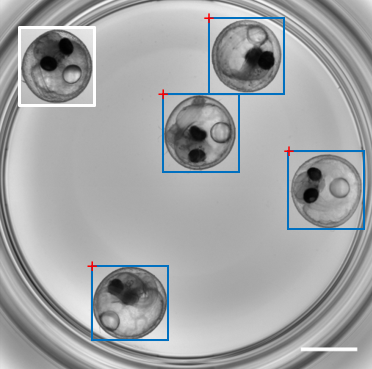
\includegraphics[width=8cm]{images/tempm.png}
	}
	\caption{Метод сопоставления с шаблоном}\label{fig:tempm}
\end{figure}

К вариации метода сопоставления с шаблоном можно отнести \textit{метод визуальных слов}. Данный метод применяется в поисковых системах и представляет каждое изображение в виде вектора параметров. Способ получения параметров может различаться, однако, часто используют поиск особых точек или дескрипторов изображений (алгоритм SIFT\footnote{Scale-Invariant Feature Transform} и его вариации), поскольку описания особой точки легко подвергаются анализу и сравнению.

\textbf{Анализ параметров объекта}. Данный метод основан на глубоком анализе параметров объекта и сравнении их с описанием эталона. Оцениваются такие данные как цвет, текстура, геометрическая форма, контур, размер, относительное расположение и другие параметры. У алгоритма нет четко выраженного шаблона объекта, но есть данные о нем, при помощи которых анализируется изображение. К примеру, известно, что объект имеет овальную форму, поэтому целесообразнее будет искать объекты овальной формы на изображении, а в дальнейшем, при помощи уточняющих признаков, определять нужный.

Одним из вариантов данного метода является, например, скелетное представление объекта. Под скелетом понимается совокупность серединных осей объекта, характеризующих его форму (рис. \cref{fig:sklt}). Данная методика требует предварительной очистки исходного изображения от шума, поскольку скелет объекта зависит от его границ, что в итоге приводит к неоднозначности определения.

\begin{figure}[ht]
	\centerfloat{
		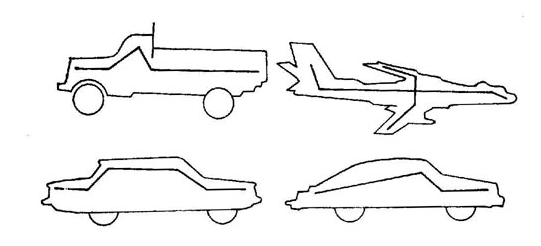
\includegraphics[width=12cm]{images/sklt.png}
	}
	\caption{Скелетное представление объектов}\label{fig:sklt}
\end{figure}

\textbf{Нейросетевой подход}. Широко распространенным сегодня методом организации распознающих систем является применение нейронных сетей. Нейронная сеть является математическим описанием взаимодействия нервных узлов живых организмов, и распознавание образов является типичной задачей для ее применения. Каждый нейрон имеет так называемый <<порог активации>>, по результату которого он принимает одно из (обычно) двух значений: 1 или 0 (-1). Помимо распознавания нейросети применяются в задачах прогнозирования, машинных переводах, улучшении и восстановлении изображений. Основная особенность нейросети --- обучение в процессе работы, которая позволяет накапливать опыт предыдущей работы для повышения точности в будущем. Также среди преимуществ применения нейросетевого подхода можно выделить высокую отказоустойчивость, быстродействие и возможность адаптации сети к изменившимся условиям. К недостаткам можно отнести долгий процесс обучения и сложность в выборе архитектуры.

Виды обучения нейросети подразделяется на обучение с учителем, без учителя и смешанное. В любом случае процесс происходит на основе датасета как можно более полного и разнообразного. К примеру, если нейросеть предназначена для распознавания текста, то в датасет загружают множество изображения букв в разных начертаниях и регистрах (рис. \cref{fig:dataset-2}). При обучении с учителем каждый элемент датасета имеет своё значение, с которым сравнивается выход нейросети, при обучении без учителя данные поставляются в сыром виде, ну а при смешанном, очевидно, одна часть данных сырая, а другая --- со значениями.

\begin{figure}[ht]
	\centerfloat{
		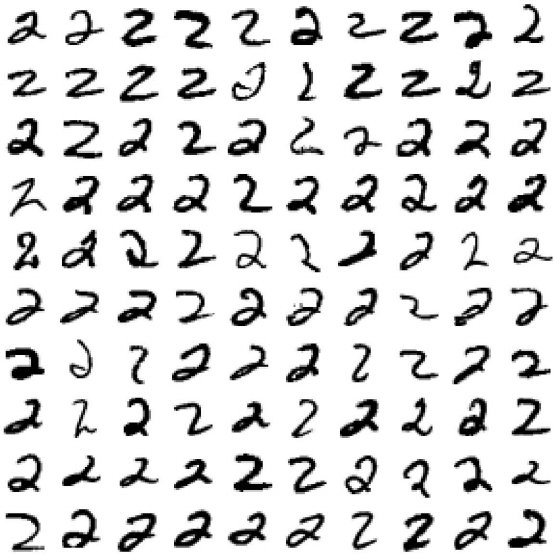
\includegraphics[width=7cm]{images/dataset-2.jpg}
	}
	\caption{Пример датасета для распознавания рукописной цифры <<2>>}\label{fig:dataset-2}
\end{figure}

Глобально нейронные сети делятся на полносвязные (обычные) и свёрточные. Полносвязные нейронные сети характеризуются тем, что каждый нейрон следующего слоя связан со всеми нейронами предыдущего, как показано на рисунке \cref{fig:pns-arch}. Сигнал в таких сетях идёт от первого слоя до последнего, без обратной связи и рекурсий, а данные на вход подаются в виде вектора, число значений в котором совпадает с числом нейронов входного слоя сети. Параметры архитектуры такой сети, то есть, количество слоёв и количество нейронов в каждом слое, почти невозможно определить, исходя только из условий задачи. К тому же, с ростом сети количество связей увеличивается экспоненциально, что затрудняет ее проектирование и затрудняет обучение.

\begin{figure}[ht]
	\centerfloat{
		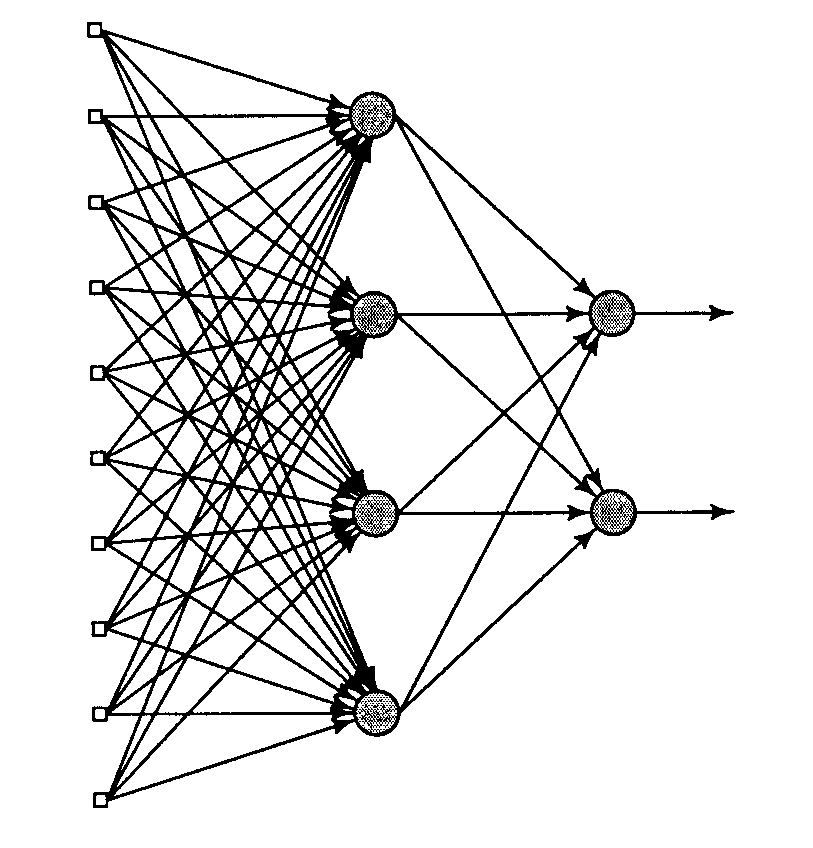
\includegraphics[width=10cm]{images/pns-arch.png}
	}
	\caption{Архитектура полносвязной нейронной сети}\label{fig:pns-arch}
\end{figure}

В свёрточных нейронных сетях, которые были описаны Яном ЛеКуном еще в 1988 году, применяется немного другой подход. В ней используется три вида слоев: свёрточные, субдескритизирующие и полносвязные. Первые два вида, свёрточные и субдескритизирующие слои, чередуются между собой для формирования входного вектора для простого полносвязного перцептрона (рис. \cref{fig:cnc-arch}). Обучение такой нейросети происходит при помощи матрицы весов (<<ядра>>), которая, перемещаясь по основному изображению, ищет присутствие некой определенной характеристики. Для этого выполняется операция свертки (чаще всего сумма произведений элементов) части изображения с весовой матрицей, формируя таким образом матрицу меньшего размера, которая затем также подвергается операции свертки с уже другой матрицей весовых коэффициентов.

\begin{figure}[ht]
	\centerfloat{
		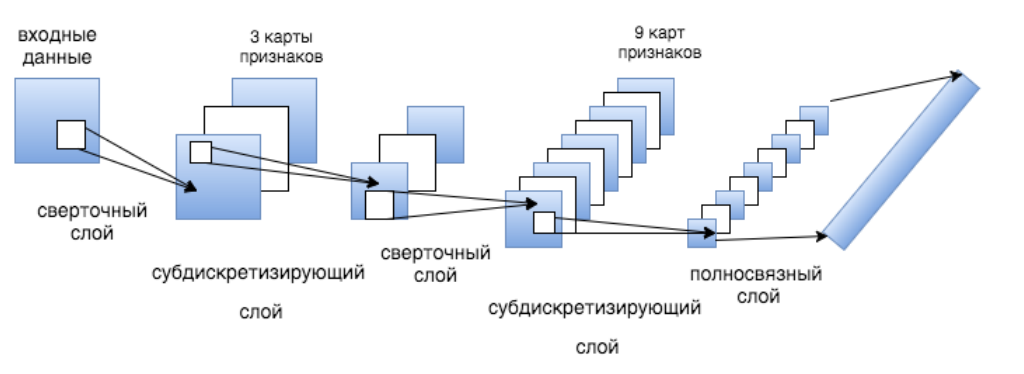
\includegraphics[width=17cm]{images/cnc-arch.png}
	}
	\caption{Архитектура сверточной нейронной сети}\label{fig:cnc-arch}
\end{figure}

В настоящее время существует множество готовых нейросетей, которые являются частью программного обеспечения или же веб-приложения. Среди сетей, нацеленных на распознавание объектов, можно назвать проект Yolo, выполняющий детектирование объектов уличного трафика. Также существует Cloud Vision API от Google, назначающий изображению ряд меток, под которые он попадает с некоторой вероятностью. Своя сеть под названием DetectNet имеется и у компании NVIDIA, она выполняет поиск объектов на основе обучающей выборки.

Тем не менее, как основной метод при проектировании СТЗ для трёхкоординатной платформы этот метод подходит лишь частично и для выполнения ряда небольших типовых задач. Поскольку условия работы оборудования отличаются непостоянством, как для составления всеобъемлющего датасета, так и для тренировки нейросети требуется затратить очень много времени. Так, в рамках исследования был опробован каскад Хаара для распознавания нескольких видов оптических меток. Входной датасет составлял 1300 <<положительных>> (содержащих метку) изображений и столько же <<отрицательных>>, то есть, не содержащих искомый объект. Все изображения были размером 320 на 240 пикселей. Обучение выполнялось для 6 видов меток, сгруппированных по двум основным типам (рис. \cref{fig:markers}):

\begin{figure}[ht]
	\centerfloat{
		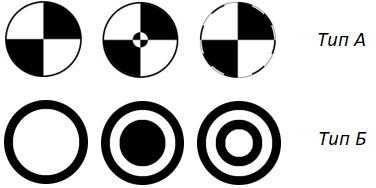
\includegraphics[width=10cm]{images/markers.png}
	}
	\caption{Метки, используемые для обучения каскада Хаара}\label{fig:markers}
\end{figure}

Метки типа А имели разбиение по четвертям круга, в том числе опциональные инвертированные сегменты для большего числа уникальных определяющих признаков, метки типа Б представляли собой устойчивые к углу поворота концентрические круги разных конфигураций. Обучение выполнялось на компьютере, обладающем следующими техническими характеристиками: два процессора Intel Xeon e5450, 32 Гб оперативной памяти, видеокарта NVidia GeForce GTS 450; видеокарта для ускорения процесса не подключалась. Время выполнения обучения для каждой метки варьировалось от 3 суток до 2 недель.

\begin{figure}[ht]
	\centerfloat{
		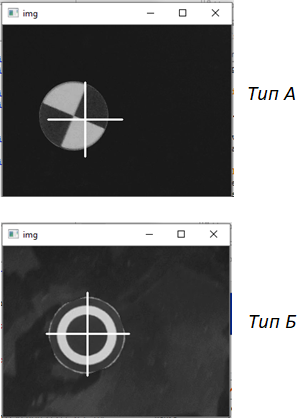
\includegraphics[width=8cm]{images/markers-res.png}
	}
	\caption{Случайным образом взятые кадры распознавания меток обоих типов}\label{fig:markers-res}
\end{figure}

Как показали результаты работы распознающей программы, в среднем у трех видов меток типа А была лишь четверть кадров, где центр метки определялся верно, а метки типа Б продемонстрировали гораздо более точный результат в 94 \% правильно обработанных кадров (рис. \cref{fig:markers-res}). Основная ошибка каскада Хаара заключалась в неверном определении границ метки, которая была вписана в большую по размеру область, из-за чего смещался найденный центр. Для меток типа А, чувствительных к масштабу и углу поворота, следовало использовать более полный датасет, учитывающий как можно больше положений метки в кадре. Однако, данный тест показал, что нейросетевой подход имеет довольно ограниченное применение в рамках задач мелкосерийного производства.

\section{Основные признаки целевых объектов} \label{sect3_2}

Задача распознавания является основой любой системы технического зрения. При проектировании основная работа приходится на процедуру описания объекта и его признаков, и чем полнее будет это описание, тем меньше ошибок при определении объекта будет совершать СТЗ. Под признаками объекта понимают некоторые его характеристики, которые участвуют в процессе распознавания, при этом стоит избегать избыточности во множестве признаков, поскольку для объекта повышается возможность отклонения вероятности наличия какого-либо признака, в результате чего он может быть проигнорирован системой. Под образом объекта подразумевается необходимо полное сочетание признаков, при которых объект будет однозначно определен.

Если принимать, что признак объекта --- это измеренная величина какой-либо характеристики объекта, то формально образ объекта будет представлять собой вектор размерности $n$, где $n$ --- количество признаков (\ref{eq_3_1}):

\begin{equation}
X = (x_1, x_2, ..., x_n)^T
\label{eq_3_1}
\end{equation}

Вектор образа объекта должен содержать, как правило, все признаки, поддающиеся измерению. В простейшем случае образы описываются как совокупность действительных числе, полученных в результате измерения образа, такие векторы стоит рассматривать как точки в $n$-мерном пространстве, а объекты одного класса будут формировать совокупность точек в области пространства с некоторым рассеянием.

Так, при сравнении двух векторов образа $X_1$ и $X_2$ выявляется некая разность $D$:

\begin{equation}
D = \|X_1 - X_2\| = \sqrt{\sum_{i=1}^{n} (X_{1i} - X_{2i})^2},
\label{eq_3_2}
\end{equation}

Соответственно, если разность $D < 2\varepsilon$, где $\varepsilon$ --- радиус окрестности усредненной (эталонной) точки из множества образов, то можно утверждать, что объект $X_2$ принадлежит к тому же классу, что и вектор объекта $X_1$.

Одна из распространенных ошибок системы распознавания --- неверная классификация, то есть, отнесение объекта к классу $\omega_i$, тогда как на самом деле объект принадлежит отличному от него классу $\omega_j$. Пусть $p(x | \omega_i) = p(X)$ --- плотность распределения вектора $X$ при условии, что он принадлежит классу $\omega_i$. Тогда вероятность принадлежности вектора к другому классу $\omega_j$ описывается как:

\begin{equation}
P = \frac{p(x | \omega_i)}{\sum_{k=1}^{m}p(x | \omega_k)},
\label{eq_3_3}
\end{equation}

где $m$ --- число классов. Данное выражение задает вероятность ошибки при определении. Соответственно, некая функция, которую называют решающей, оптимальна в том случае, если соблюдается неравенство:

\begin{equation}
p(x | \omega_i) > p(x | \omega_j) \forall i \neq j
\label{eq_3_4}
\end{equation}

Очевидно, что далеко не все признаки объекта можно измерить при помощи визуального анализа. Также очевидно и то, что некоторые характеристики объекта не могут быть выражены в форме действительных чисел, представляя собой функцию, определенную на некотором пространстве. В общем виде признаки на изображении могут быть разделены на 4 подгруппы \cite{Myasnikov}.

Простейшим видом признаков объектов являются \textbf{геометрические}. К этому классу признаков относится не только непосредственно форма объекта, но и его расстояние от другого объекта, центр масс, площадь объекта и т.д. Однако, чаще всего речь идет о контурном анализе, поскольку контур объекта --- наиболее важных и наглядных характеристик объекта. Метод описания контура объекта при помощи цепного кода был предложен Фриманом в 1961 году. В его основе лежит описание контура как последовательности численных значений направлений каждой следующей точки контура. Таким образом, метод является простым в организации и полезным для получения сопутствующих характеристик объекта, но слабо устойчивым к искажениям изображения.

Другая группа признаков объекта --- \textbf{топологические признаки}, то есть, ряд признаков, остающихся неизменными относительно топологии объекта. Само по себе топологическое отображение объекта малоинформативно, поскольку топологическое описание объекта не характеризует его геометрическую форму. Для того, чтобы полно описать объект, необходим расчет топологических признаков, таких, как число отверстий или связных компонентов в объекте. Эти расчеты достаточно сложны, поэтому топологические признаки применяются на практике достаточно редко.

\textbf{Вероятностные признаки} отражают модель распределения яркости на изображении, к которым относятся гистограмма распределения яркости, моменты изображения и стохастическая геометрия. Особый интерес в данной группе признаков представляют моменты изображения. С помощью моментов описывается центр масс изображения, а также его ориентация в пространстве относительно осей. Пусть дано следующее выражение:

\begin{equation}
M_0 = m_1 + m_2 + ... + m_n = \sum_{i=1}^{n} m_i,
\label{eq_3_5}
\end{equation}

где $M_0$ --- площадь изображения (так называемый <<нулевой момент>>), $m_1, ..., m_n$ --- площади элементов изображения, полученных при сегментации, $n$ --- количество сегментов. Главные осевые моменты изображения будут представлять собой моменты первого порядка $M_{1x}$ и $M_{1y}$:

\begin{equation}
M_{1x} = m_1 x_1 + m_2 x_2 + ... + m_n x_n = \sum_{i=1}^{n} m_i x_i,
\label{eq_3_6}
\end{equation}

\begin{equation}
M_{1y} = m_1 y_1 + m_2 y_2 + ... + m_n y_n = \sum_{i=1}^{n} m_i y_i,
\label{eq_3_7}
\end{equation}

Моменты первого порядка изображения позволяют вычислить точку расположения центра тяжести изображения:

\begin{equation}
X_0 = \frac{M_{1x}}{M_0}, Y_0 = \frac{M_{1y}}{M_0}.
\label{eq_3_8}
\end{equation}

Моменты второго порядка позволяют определить признаки изображения, инвариантные к сдвигу и повороту, а также направление главных осей изображения:

\begin{equation}
M_{2x} = m_1 x_1^2 + m_2 x_2^2 + ... + m_n x_n^2 = \sum_{i=1}^{n} m_i x_i^2,
\label{eq_3_9}
\end{equation}

\begin{equation}
M_{2y} = m_1 y_1^2 + m_2 y_2^2 + ... + m_n y_n^2 = \sum_{i=1}^{n} m_i y_i^2,
\label{eq_3_10}
\end{equation}

Или, в более общем виде:

\begin{equation}
M_k = \sum_{i=1}^{n} m_i x_i^k y_i^p,
\label{eq_3_11}
\end{equation}

где $k$ и $p$ --- показатели степеней, $k,p\in[1, n]$.

Помимо определения характеристик изображения, моменты используются для сравнения, например, контуров, однако, моменты первого порядка при всей простоте вычисления не позволяют сравнивать между собой контуры одинаковой формы, но разных размеров.

Наконец, \textbf{спектральные признаки}, для определения которых используется модель спектрального преобразования:

\begin{equation}
g(m_1, m_2) = \sum_{N_1 - 1}^{i = 0} \sum_{N_2 - 1}^{j = 0} f(i, j) W(i, j, m_1, m_2),
\label{eq_3_12}
\end{equation}

где $W(\cdot)$ --- ядро преобразования, которое зависит от выбранного типа преобразования (Карунена-Лоэва, Фурье, косинусное и т.д.).

\section{Анализ и синтез алгоритмов обработки изображений} \label{sect3_3}

\subsection{Общая постановка задачи} \label{ssect3_3_1}

Очевидно, что технологическое оборудование отличается полнотой списка выполняемых на нем операций, что делает невозможным использование какой-то одной теории для построения взаимодействия систем. Рассматриваемый процесс проектирования СТЗ для трёхкоординатной платформы опирается на несколько базисов. Во-первых, имеет место неоднородность решаемых задач с уклоном в класс контролирующих операций. Во-вторых, СТЗ должна пользоваться не только результатами визуального анализа, но и другой вспомогательной информацией и реагировать на изменения в техпроцессе. В-третьих, СТЗ должна иметь двустороннее сообщение с системой управления платформы и выдавать данные в подготовленном для работы платформы виде.

В первую очередь, необходимо разделить целевые объекты на классы. В рамках производства можно выделить следующие классы:

\begin{enumerate}
	\item Отверстия.
	\item Пазы.
	\item Дорожки.
	\item Силуэт детали.
	\item Силуэт элемента детали.
	\item Пятно лазера.
	\item Оптические метки.
\end{enumerate}

Соответственно, данное распределение по классам представляет собой минимальное описание рассматриваемой номенклатуры изготавливаемых изделий и является основой для описания СТЗ. Согласно изложенному выше, каждый класс объектов имеет ряд признаков, не пересекающийся с рядом признаков любого другого класса. Таким образом, пусть $\Omega = (\omega_1, ..., \omega_k)$ --- множество рассматриваемых классов, $C = (c_1, ..., c_l)$ --- множество объектов, принадлежащих одному классу, $f(C_x) \to \omega_i$ и $f(C_y) \to \omega_j$ --- функция соответствия векторов объектов $C_x = (x_1, ..., x_n)$ и $C_y = (y_1, ..., y_m)$ классам $\omega_i$ и $\omega_j$ соответственно. При этом должны соблюдаться условия:

\begin{equation}
C_i \cap C_j = \emptyset,
\label{eq_3_13}
\end{equation}

\begin{equation}
\forall C: C \in \omega_i, i = [1, k], \nexists f(C) \to \omega_j, j \neq i,
\label{eq_3_14}
\end{equation}

\begin{equation}
\forall c_i: c_i \in C_j, i=[1, l], j=[1, k], \nexists C_k \supset c_i, k \neq j.
\label{eq_3_15}
\end{equation}

Выбор подходящего класса объекта основывается исключительно на его совокупной группе признаков. Этот же принцип должен лежать в основе программного описания объектов конкретного класса и работы с ними.

Выбор работы с конкретным классом объектов определяется из первичного анализа управляющей программы, в нужный момент должны запускаться соответствующие функции ПО и строго в свою очередь, более того, это же относится и к объектам одного класса с разными параметрами. Таким образом, невозможно создать неопределенность, когда СТЗ вынуждена работать одновременно с двумя и более разными объектами, повышая вероятность появления ошибки неверного распознавания. Пусть $g(C_i) \to t_i$ и $g(C_j) \to t_j$ --- время начала выполнения операций над объектами $C_i$ и $C_j$, а $\delta t_i$ --- время выполнения операции над объектом $C_i$ до перехода к объекту $C_j$. Тогда должны выполняться условия:

\begin{equation}
\delta t_i \leq |t_j - t_i|, i < j,
\label{eq_3_16}
\end{equation}

\begin{equation}
\forall C_i: C_i, i = [1, l], \exists g(C_i) \to t_i \neq t_j, i \neq j.
\label{eq_3_17}
\end{equation}

Кроме того, полагая, что $h(C_i) \to O_i$ --- тип операции, производимой над объектом $(C_i)$, то должно соблюдаться:

\begin{equation}
h(C_i) \to O_i \neq h(C_j) \to O_j, j \neq i,
\label{eq_3_18}
\end{equation}

\begin{equation}
\forall C_i: C_i \in \omega_j, i = [1, n], j = [1, m], \nexists h(C_i) \to O_k, k \neq i.
\label{eq_3_19}
\end{equation}

Таким образом исключается возможная неоднозначность в одинаковых операциях над разными типами объектов.

Пусть $Z_0$ --- число объектов одного типа в кадре, а $Z$ --- максимум одновременно обрабатываемых объектов одного типа, тогда должно соблюдаться:

\begin{equation}
\forall i: i=[1, k], \frac{g(C_i | \delta t_i)}{\gamma} \leq Z_0, \gamma = \frac{g(C_i | \delta t_i)}{Z},
\label{eq_3_20}
\end{equation}

\subsection{Базовые задачи, выполняемые СТЗ для трехкоординатной платформы} \label{ssect3_3_2}

Рассматривая постановку задачи далее, можно приступить к описанию более конкретных базовых функций СТЗ, то есть, тех, которые не требуют подключения дополнительных сенсоров. Очевидно, что все задачи СТЗ должны иметь жестко определенный перечень операций, а также соответствовать ограничениям и условиям, описанным ранее.

\textbf{Определение нуля заготовки}. Данная задача выполняется для корректировки положения инструмента перед началом выполнения следующего за ним сегмента УП. Необходимость наличия этой операции обусловлена погрешностями установки заготовки на рабочую поверхность платформы. После выявления нулевой точки заготовки каретка трехкоординатной платформы должна сдвинуться в указанную позицию так, чтобы ось инструмента и нулевая точка заготовки совпали с требуемой точностью. Поиск метки на заготовке осуществляется с применением к кадрам градиентного фильтра и последующей пороговой бинаризации.

\textit{Входные данные}: заготовка с нанесенными при помощи УФ-принтера оптическими метками.

\textit{Выходные данные}: измеренные расстояния сдвига каретки платформы по осям $x$ и $y$.

\textit{Порядок операций}:

\begin{enumerate}
	\item Получение команды на выставление нуля заготовки.
	\item Проверка готовности контроллера СТЗ к работе путем его опрашивания посредством ЛВС.
	\item Отведение каретки в дальнюю позицию платформы. Это необходимо для исключения вероятности загораживания меток на заготовке элементами платформы.
	\item Включение обзорной камеры, поиск заготовки на рабочей поверхности посредством обработки кадра, возврат области рабочей поверхности.
	\item Перемещение каретки в указанную область. 
	\item Включение дополнительной камеры на модуле, поиск метки на заготовке посредством обработки не менее 5 кадров.
	\item Вычисление расстояния через связь <<пиксель --- миллиметр --- шаг энкодера>>.
	\item Перемещение каретки в рассчитанную точку.
	\item Сигнал о готовности, переход к выполнению сегмента УП.
\end{enumerate}

\textit{Требуемая точность выставления}: $\pm$100 мкм.

\textbf{Соотнесение оси подключенного модуля с системой координат платформы}. Выполняется при подключении нового модуля к каретке. Поскольку модули могут отличаться по своим габаритным размерам в зависимости от вида инструмента, в регистре описания модуля должен содержаться параметр расстояния от оси инструмента до угловой метки, нанесенной сверху на модуль. Таким образом, после сопряжения систем координат, положение оси инструмента должно совпадать с нулевой точкой платформы с заданной точностью.

\begin{figure}[ht]
	\centerfloat{
		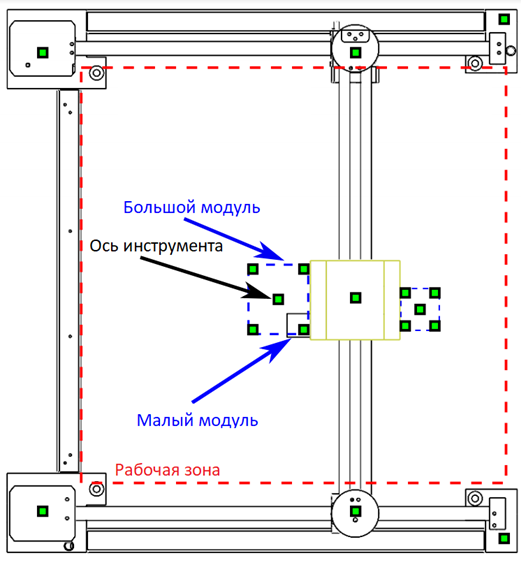
\includegraphics[width=11cm]{images/posit.png}
	}
	\caption{Схема размещения оптических маркеров на рабочей области}\label{fig:posit}
\end{figure}

\textit{Входные данные}: Оптические метки, нанесенные на направляющую, на углы рабочей области, и на угол подключенного модуля, согласно схеме, представленной на рисунке \cref{fig:posit}.

\textit{Выходные данные}: Глобальные координаты в УП и координаты инструменты должны совпасть между собой.

\textit{Порядок операций}:

\begin{enumerate}
	\item Установка модуля и его регистрация в системе управления.
	\item Получение расстояния от угловой метки модуля до оси инструмента.
	\item Смещение каретки платформы в центр рабочей области платформы.
	\item Включение обзорной камеры, снимок обзорной камерой для определения параметров рабочей зоны.
	\item Включение дополнительной камеры на модуле.
	\item Перемещение каретки в нулевую, в дальнюю и снова в центральную позицию платформы, определение угловых меток рабочей области платформы.
	\item Вычисление соотношения между метками и перемещениями энкодера.
	\item Вычисление сдвига относительно угловой метки модуля.
	\item Сигнал о готовности и выполнение следующего сегмента УП.
\end{enumerate}

\textit{Требуемая точность выставления}: $\pm$100 мкм.

\textbf{Периодический контроль положения заготовки на рабочей поверхности}. Данная задача необходима для периодической проверки на отсутствие перемещений заготовки по рабочей зоне в ходе выполнения над ней обрабатывающих операций. Таким образом уменьшается количество неверно обработанных заготовок. Данная задача выполняется через сравнение кадра с так называемым эталонным кадром.

\textit{Входные данные}: Эталонный кадр с обзорной камеры, который выполняется при установке заготовки, а также вычисления её нуля с передачей снимка контроллеру СТЗ.

\textit{Выходные данные}: Сигналы о готовности продолжения обработки заготовки, передаваемые контроллеру платформы.

\textit{Порядок операций}:

\begin{enumerate}
	\item Установка заготовки на рабочую поверхность платформы.
	\item Вычисление нуля заготовки.
	\item Выполнение серии снимков рабочей области обзорной камерой и передача усредненного снимка на контроллер СТЗ.
	\item Получение команды из УП на проверку положения заготовки.
	\item Выполнение серии снимков обзорной камерой и передача усредненного снимка на контроллер СТЗ.
	\item Сравнительный анализ полученного снимка с эталонным с вычислением отклонения объектов.
	\item При отсутствии отклонения (не более 1 пикселя сдвига) передача сигнала о готовности продолжать работу.
	\item При наличии отклонения приостановка выполнения УП, ожидание исправления положения заготовки с последующим определением ее нулевой точки.
\end{enumerate}

\textit{Требуемая точность сравнения}: не более 1 пикселя сдвига.

\subsection{Расширенные задачи, требующие дополнительных модулей для СТЗ} \label{ssect3_3_3}

Помимо вышесказанного, очевидно, что в рамках различных технологических процессов, выполняющихся на платформе, могут разниться условия работы и требования к конечному изделию. Соответственно, могут возникать ситуации, когда информации, получаемой от обзорной и вспомогательной камер, может оказаться недостаточно. Это касается не только требований к изделию, но так же к усилению контроля над заготовкой и инструментом. В данном случае описанная в 1 главе концепция модульного оборудования должна распространяться и на СТЗ, позволяя подключать к ней вспомогательные устройства и датчики.

Представление таких модулей в системе слабо отличается от инструментальных. У них так же имеется запись в реестре, описывающая их характеристики: имя в сети, выполняемые функции, команды в УП. Между ними и центральным узлом СТЗ, роль которого обычно исполняет обрабатывающий контроллер СТЗ, должна быть свободная двусторонняя связь, посредством которой центральный узел принимает данные в том виде, в каком их посылает сенсор, и при этом может обратиться к сенсору при помощи сигналов включения/отключения, удалённого изменения параметров или изменения формата предоставляемых данных. Схема взаимодействия модулей представлена на рисунке \cref{fig:posit}.

\begin{figure}[ht]
	\centerfloat{
		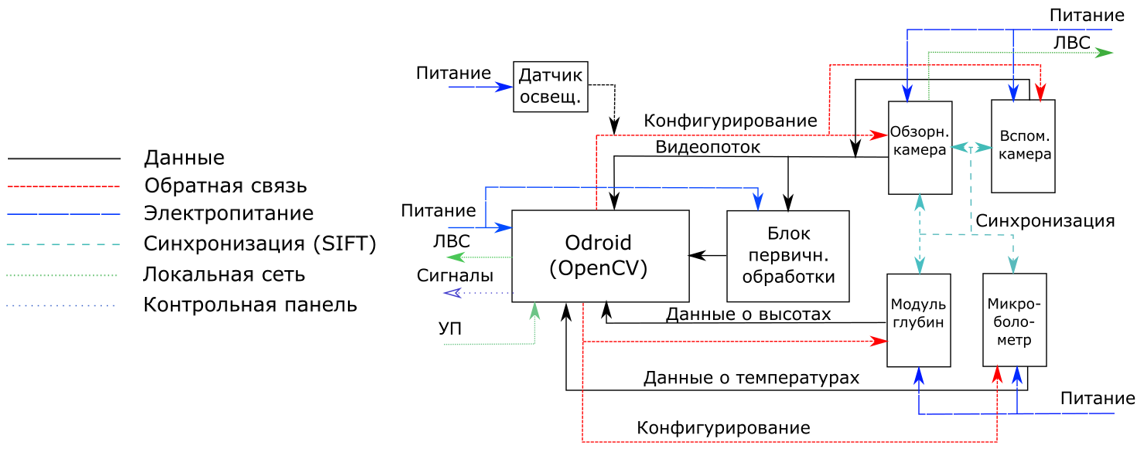
\includegraphics[width=\textwidth]{images/dop-scheme.png}
	}
	\caption{Схема взаимодействия вспомогательных датчиков в СТЗ}\label{fig:dop-scheme}
\end{figure}

В работе многосенсорной СТЗ необходимо обеспечить единство поступающей информации. Для этого служит операция синхронизации нескольких камер, расположенных в разных точках рабочей области. Синхронизация осуществляется путем вычисления соответственных точек при помощи алгоритма SIFT и построения с их помощью связи между двумя и более изображениями.

Таким образом, алгоритм взаимодействия СТЗ со вспомогательными сенсорами во время технологического процесса выглядит следующим образом. Сперва выполняется анализ обработчиком входной управляющей программы на предмет состава операций и необходимого оборудования. Затем диспетчер платформы опрашивает все модули в сети, составляя таким образом список устройств и ожидая подключения нужных, если какой-то модуль оказался не найден. Далее выполняется первоначальная удалённая конфигурация сенсоров, им передаются необходимые значения параметров работы, выполняется синхронизация модулей через алгоритм поиска особых точек. После этого составляются основные этапы алгоритма работы СМЗ и начинается выполнение техпроцесса, во время которого модули так же могут удаленно конфигурироваться, если это необходимо. Среди передаваемых параметров могут быть координаты области кадра, интервал температур, интервалы высот и так далее.

Даже смартфоны сейчас уже не обходятся только одной камерой и имеют два или более объектива вместе с дополнительными сенсорами. Это позволяет существенно увеличить возможности съемки фотографий, получать более сложные кадры. Это же применимо и к компоненту СТЗ оборудования. Среди простых вспомогательных сенсоров можно выделить следующие:

\begin{enumerate}
	\item Датчик освещенности рабочего пространства для выправления баланса белого. Данный сенсор может располагаться рядом с обзорной камерой, но для лучшего применения должно быть размещено несколько таких датчиков в разных участках рабочего пространства.
	\item Микроболометр предоставляет информацию о температурах изделия и инструмента во время обработки. Соответственно, его логичнее располагать сбоку под углом, чтобы был виден и инструмент, и заготовка.
	\item Проектор размерной сетки на рабочую область применяется в задачах контроля положения заготовки или выделения области обработки, в которую нельзя заходить инструменту. Модуль должен располагаться сверху, рядом с обзорной камерой, однако, проецируемые линии могут перекрываться кареткой.
	\item Из-за повышенной концентрации частиц в воздухе видимость может ухудшаться, так что иногда необходим датчик для их контроля.
	\item Модуль глубины изображения, основанный на лазерном сканировании сцены с определением времени возврата луча и возвращает массив из численных значений расстояния от линзы до объекта. Однако, модуль глубин имеет достаточно ограниченное применение в оборудовании. Например, при помощи него можно составить грубую карту высот, которая понадобится для расчёта безопасной траектории инструмента без задевания заготовки. Также им можно отсеивать нужные области кадра по указанному интервалу высот. Но существует ряд недостатков, среди которых можно выделить плохую восприимчивость некоторых типов поверхностей, потребность в начальной привязке модуля глубин в какой-нибудь плоскости и т.д.
\end{enumerate}

\subsection{Унификация алгоритмов} \label{ssect3_3_4}

Очевидно, что в рамках широкого применения СТЗ важным фактором является единство описания модулей и простота их вызова в программе-обработчике. Помимо работы непосредственно с камерой необходимы функции для работы со вспомогательными модулями. Иными словами, для разработки ПО для СТЗ требуется использование единой программной среды. Это обусловлено также и необходимостью дальнейшей поддержки и расширения функций СТЗ.

Существует несколько многофункциональных решений с открытым исходным кодом от разных фирм. К примеру, свой SDK\footnote{Пер. с англ. --- Набор для разработки программного обеспечения} для работы с разными модулями есть у производителя камер Intel Realsense, который в настоящее время активно улучшается и пополняется. Также есть библиотека для работы с оборудованием для дополненной реальности от ARCore. Кроме того, можно упомянуть производителя разного рода оптических сенсоров FRAMOS.

Необходимый для работы список дополнительного оборудования должен определяться, исходя из анализа УП обрабатывающим контроллером. На основе этого списка ПО станка генерирует программу для СТЗ с нужной последовательностью работы и с параметрами, также взятыми из УП.

\subsection{Методика измерений} \label{ssect3_3_5}

Использование СТЗ в качестве средства измерения какого-либо размера изделия имеет как достоинства, так и недостатки по сравнению с ручным измерением при помощи штангенциркулей, микрометров и других приборов. Очевидно, что ручное измерении большой партии изделий занимает много времени, а выборочная проверка части изделий из партии не гарантирует отсутствие брака. Автоматизация этого процесса позволяет повысить эффективность производства и снизить временные затраты на контроль. В противовес этому, СТЗ не может обеспечивать микронной точности измерения, поскольку имеет ограничение на уровне пикселей изображения. Попытка увеличить разрешение изображения приводит к увеличению затрат ресурсов обрабатывающего компьютера, установке камер с более высокой разрешающей способность и, как следствие, удорожанию всей СТЗ. Основным стандартом, регламентирующим методики измерений при помощи СТЗ, является EMVA 1288, разработанный в 2010 году \cite{emva1288}.

Логично, что проще всего определить размер объекта на изображении можно при помощи метода нахождения краёв объекта. Здесь сопоставляется размер изображения и количество пикселей, укладывающихся в длину объекта. Таким образом, разрешение пикселей камеры рассчитывается в мм/пкс по формуле \cite{eq_3_25}:

\begin{equation}
R = \frac{h}{n} \cdot tg(\frac{\alpha}{2}),
\label{eq_3_25}
\end{equation}

где $h$ --- высота от линзы до объекта (фокусное расстояние) в мм, $n$ --- ширина (или высота) кадра в пикселях, $\alpha$ --- угол поля зрения камеры по ширине или по высоте в градусах. Отсюда можно рассчитать фактическое поле допуска камеры при измерениях. Расчёт основан на предположении, что поле допуска должно в 10 раз превышать повторяемость СТЗ, которая на практике обычно равна 0,5 пикселя \cite{Nello2000}. Таким образом, поле допуска составляет $\pm5$ пикселей. Для конкретной разрешающей способности оно будет рассчитываться:

\begin{equation}
D = 5 \cdot R,
\label{eq_3_26}
\end{equation}

Например, величины поля допуска на размер для камеры формата FullHD (1080p) при высоте в 500 мм и поле зрения в 115 градусов по горизонтали и 65 градусов по вертикали будут составлять 2,04 мм по горизонтали и 1,47 мм по вертикали.

Тем не менее, с использованием обработки изображений можно получить расстояния в долях пикселя. Для этого необходимо при обнаружении края объекта провести дифференциальную обработку яркости данного пикселя и, на основании распределения яркостей, получить пиковое значение \cite{fig:subpixel-count} \cite{web:dimention}.

\begin{figure}[ht]
	\centerfloat{
		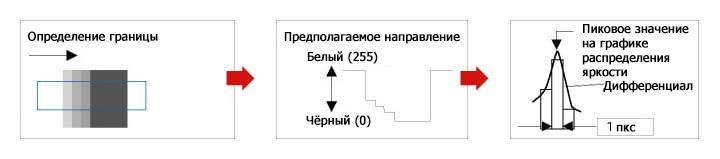
\includegraphics[width=\textwidth]{images/subpixel-count.png}
	}
	\caption{Алгоритм обработки субпикселей}\label{fig:subpixel-count}
\end{figure}

\section{Метрологическое обеспечение измерительных систем с использованием технического зрения} \label{sect3_4}

Поскольку проектируемая СТЗ может выполнять в том числе и измерительные функции, к ней применяется процедура установления метрологического обеспечения. Потребность в предоставлении достоверных данных измерения прямым образом влияет на качество конечного изделия, а также на необходимость последующей доработки изделия перед сбытом и вводом в эксплуатацию. СТЗ функционирует как автоматизированная измерительная система (АИС), то есть, представляет собой комплекс измерительных средств, расположенных в разных точках пространства и обменивающийся информацией по внутренним каналам связи. Как автоматизированная информационная система, СТЗ регламентируется стандартами:

\begin{itemize}
	\item ГОСТ Р 8.596-2002 <<Государственная система обеспечения единства измерений (ГСИ). Метрологическое обеспечение измерительных систем. Основные положения>>,
	\item ГОСТ 8.009-84 <<Государственная система обеспечения единства измерений (ГСИ). Нормируемые метрологические характеристики средств измерений>> (межгосударственный),
	\item ГОСТ 34.201-89 <<Информационная технология. Комплекс стандартов на автоматизированные системы. Виды, комплектность и обозначение документов при создании автоматизированных систем>>,
	\item ГОСТ 34.601-90 <<Информационная технология. Комплекс стандартов на автоматизированные системы. Автоматизированные системы. Стадии создания>>,
	\item ГОСТ 27300-87 <<Информационно-измерительные системы. Общие требования, комплектность и правила составления эксплуатационной документации>>.
\end{itemize}

Исходя из этого, необходимо представить перечень характеристик СТЗ, подлежащих нормированию согласно вышеуказанным стандартам.

\textbf{Измерение габаритов заготовки стандартное простое, на высоте до 750 мм}. Выполняется пересчёт области кадра в метрическую систему посредством соотношения <<пиксель-миллиметр>>. Номинальная функция преобразования:

\begin{equation}
Y = X \cdot \frac{h / cos (\alpha / 2)}{0,5 \cdot X_0},
\label{eq_3_21}
\end{equation}

где $Y$ --- величина измерения в мм, $X$ --- величина измерения в пикселях, $X_0$ --- ширина кадра в пикселях, $\alpha$ --- угол поля зрения камеры по горизонтали или вертикали, $h$ --- высота расположения камеры в мм.

Вид выходного кода представлен в виде натурального десятичного числа с плавающей запятой.

Систематическая погрешность $\Delta_s$ измерения составляет $\pm$500 мкм.

Случайная погрешность $\Delta_o$ измерения составляет $\pm$ мкм.

\textbf{Измерение высоты от верхней поверхности заготовки до линзы}. Выполняется путём расчёта времени возврата лазерного луча с фиксированным значением скорости прохождения в нормальных условиях. Номинальная функция преобразования:

\begin{equation}
Y = \frac{2 \cdot c}{t},
\label{eq_3_22}
\end{equation}

где $Y$ --- величина измерения в мм, $c$ --- скорость распространения лазерного луча в нормальных условиях, $t$ --- время, проходящее от момента испускания до момента поглощения вернувшегося луча.

Систематическая погрешность $\Delta_s$ измерения составляет $\pm$500 мкм.

Случайная погрешность $\Delta_o$ измерения составляет $\pm$ мкм.

\textbf{Измерение освещенности рабочего пространства}. Выполняется при помощи светочувствительных датчиков, расположенных в разных точках рабочей области платформы. Номинальная функция преобразования:

\begin{equation}
Y = \frac{1}{N} \sum_{i=1}^{N} \delta \Phi_i,
\label{eq_3_23}
\end{equation}

где $Y$ --- величина измерения в люксах, $N$ --- количество датчиков в рабочем пространстве, $\Phi_i$ --- световой поток, замеренный одним датчиком.

Систематическая погрешность $\Delta_s$ измерения составляет 15~\%.

Случайная погрешность $\Delta_o$ измерения составляет .

\textbf{Измерение температуры в указанной точке кадра}. Выполняется посредством микроболометра, выполняющего операцию перевода испускаемого объектом ИК-излучения в величину температуры в градусах Цельсия. Номинальная функция преобразования:

\begin{equation}
Y = \frac{C}{\lambda P}, P = ln[1 + \frac{kC_0}{\lambda^5 \cdot I_\lambda (\lambda)}] + 273,15,
\label{eq_3_24}
\end{equation}

где $Y$ --- величина измерения в градусах Цельсия, $C$ = 14387,8 мкм$\cdot$К, $\lambda$ --- длина волны излучения точки, $k$ --- коэффициент преобразования для регистрируемого излучения, $C_0$ = 37417,7 Вт$\cdot$мкм$^4$, $I_\lambda$ --- удельная спектральная мощность по длинам волн (Вт$\cdot$мкм$^4$$\cdot$см$^{-2}$).

Систематическая погрешность $\Delta_s$ измерения составляет 2,5~\%.

Случайная погрешность $\Delta_o$ измерения составляет .

%\section{Анализ эффективности применения систем технического зрения} \label{sect3_5}

\section{Выводы по третьей главе} \label{sect3_6}

В данном разделе были рассмотрены основные методы построения СТЗ для какой-то конкретной задачи. В индустрии широко находят применение как классические методы, основанные на обработке изображений, так и применение нейросетевого подхода. Каждый подход к организации имеет свои преимущества и недостатки, однако, для модульной трёхкоординатной платформы для мелкосерийного производства лучше всего подходит именно первый класс методов, как более гибкий и настраиваемый.

Далее было сформировано представление объекта и его признаков в формализованной форме. Существуют разные виды признаков изображений и чаще всего на практике применяется их комбинация. Однако, следует избегать избыточности описания объекта в системе, поскольку это усложняет методы распознавания, а некоторые объекты по ряду признаков могут пересекаться с другими.

Также была сформулирована общая задача построения и функционирования СТЗ в системе управления трёхкоординатной платформы. В качестве общих условий были прописаны основные правила и ограничения на функционирование компонентов СТЗ, а также рассмотрены сами функции с порядком действий, входными и выходными параметрами. Практическое представление данного раздела будет рассмотрено далее в следующей главе.

Наконец, было уделено внимание метрологической составляющей. В соответствующем разделе представлены измеряемые при помощи СТЗ величины вместе с формулами для их расчета. Достоверность получаемых от СТЗ данных напрямую влияет на её функционирование и конечное качество продукта, поэтому данному вопросу также стоит уделить внимание.           % Глава 3
\chapter{Аппаратная и программная составляющая систем машинного зрения} \label{chapt4}

\section{Обоснование выбора технических средств} \label{sect4_1}

12

\section{Обзор и обоснование выбора программных средств} \label{sect4_2}

\section{Описание структуры модуля машинного зрения} \label{sect4_3}

\section{Выводы по четвертой главе} \label{sect4_4}           % Глава 4
\chapter*{Заключение}                       % Заголовок
\addcontentsline{toc}{chapter}{Заключение}  % Добавляем его в оглавление


      % Заключение
\chapter*{Список сокращений и условных обозначений} % Заголовок
\addcontentsline{toc}{chapter}{Список сокращений и условных обозначений}  % Добавляем его в оглавление
% при наличии уравнений в левой колонке значение параметра leftmargin приходится подбирать вручную
\begin{description}[align=right,leftmargin=3.5cm]
\item[АИС] автоматизированная измерительная система
\item[АТС] автономное (беспилотное) транспортное средство
\item[ИК] инфракрасный (диапазон)
\item[ЛВС] локальная вычислительная сеть
\item[ПЛК] программируемый логический контроллер
\item[ПО] программное обеспечение
\item[СПФ] сухой пленочный фоторезист
\item[СТЗ] система технического зрения
\item[ЧПУ] числовое программное управление
\item[УП] управляющая программа
\item[BSD] Berkeley Software Distribution
\item[GPL] General Public License
\item[GPU] Graphics Processing Unit, блок вычисления графики
\item[JSON] JavaScript Object Notation
\item[OEE] Overall Equipment Efficiency, показатель общей эффективности оборудования.
\item[QR] Quick Response (code)
\item[RDP] Remote Desktop Protocol, протокол для удалённого доступа к компьютеру посредством ЛВС от Microsoft
\item[SDK] Software Developer's Kit, набор для разработки ПО.
\item[SIFT] Scale-Invariant Feature Transform
\item[VNC] Virtual Network Computing, протокол для удалённого доступа к компьютеру посредством ЛВС от Oracle
\end{description}
        % Список сокращений и условных обозначений
\chapter*{Словарь терминов}             % Заголовок
\addcontentsline{toc}{chapter}{Словарь терминов}  % Добавляем его в оглавление

\textbf{Автономное транспортное средство} : вид транспортных средств, перемещающихся без участия человека, используя геолокацию или систему технического зрения

\textbf{Захват изображения} : процесс фиксации входного видеопотока при помощи датчика изображения с последующим преобразованием в цифровой формат

\textbf{Объект} : предмет или часть предмета из реального мира или какой-то его параметр

\textbf{Пиксель} : минимальная составляющая цифрового изображения

\textbf{Программируемый логический контроллер} : разновидность электронной вычислительной машины для выполнения специализированных задач, чаще всего, в области автоматизации технологических процессов

\textbf{Стартап} : разновидность формы организации компании, целью которой является поиск воспроизводимой бизнес-идеи или обкатка какой-либо инновации на рынке      % Словарь терминов
\include{Dissertation/references}      % Список литературы
\include{Dissertation/lists}           % Списки таблиц и изображений (иллюстративный материал)

\setcounter{totalchapter}{\value{chapter}} % Подсчёт количества глав

%%% Настройки для приложений
\appendix
% Оформление заголовков приложений ближе к ГОСТ:
\setlength{\midchapskip}{20pt}
\renewcommand*{\afterchapternum}{\par\nobreak\vskip \midchapskip}
\renewcommand\thechapter{\Asbuk{chapter}} % Чтобы приложения русскими буквами нумеровались

%\include{Dissertation/appendix}        % Приложения

\setcounter{totalappendix}{\value{chapter}} % Подсчёт количества приложений

\end{document}
